% ============================================================
%  Vertex — Milestone 1 Report
%  Operating Systems Course Project
%  Team: Muhammad Roohullah (27082), Hayatullah (23035), Sudharth Kumar (26925)
%  Repository: https://github.com/Moorani/xv6-distributed-inference
%
%  COMPILE:
%    pdflatex Vertex_Report_Milestone1.tex
%    pdflatex Vertex_Report_Milestone1.tex   (twice, for TOC + refs)
%
%  EXPECTED FILES IN THE SAME DIRECTORY:
%    figures/F1.png ... F7d.png   (rendered Mermaid diagrams)
%    figures/warmup_callgraph.png
%    figures/transcript_single.png
%    figures/transcript_ring2.png
%    figures/transcript_ring3.png
%    figures/transcript_weightfetch.png
%    figures/transcript_allthree.png
%  If a figure is missing, replace \includegraphics with \fbox{\parbox{...}{...}}
% ============================================================

\documentclass[11pt,a4paper]{article}

% ---------- Core packages ----------
\usepackage[utf8]{inputenc}
\usepackage[T1]{fontenc}
\usepackage[margin=1in]{geometry}
\usepackage{graphicx}
\usepackage{booktabs}
\usepackage{longtable}
\usepackage{tabularx}
\usepackage{array}
\usepackage{multirow}
\usepackage{amsmath,amssymb}
\usepackage{enumitem}
\usepackage{float}
\usepackage{caption}
\usepackage{subcaption}
\usepackage{xcolor}
\usepackage{listings}
\usepackage{fancyhdr}
\usepackage{titlesec}
\usepackage[hidelinks]{hyperref}
\usepackage{parskip}

% ---------- Page style ----------
\pagestyle{fancy}
\fancyhf{}
\rhead{Vertex --- Milestone 1}
\lhead{Distributed Inference on xv6-RISC-V}
\cfoot{\thepage}
\renewcommand{\headrulewidth}{0.4pt}

% ---------- Code listings ----------
\definecolor{codebg}{RGB}{245,245,245}
\definecolor{codekw}{RGB}{0,0,160}
\definecolor{codecm}{RGB}{0,128,0}
\definecolor{codestr}{RGB}{170,0,0}
\lstset{
  basicstyle=\ttfamily\small,
  breaklines=true,
  frame=single,
  backgroundcolor=\color{codebg},
  keywordstyle=\color{codekw},
  commentstyle=\color{codecm},
  stringstyle=\color{codestr},
  showstringspaces=false,
  columns=fullflexible,
  keepspaces=true,
  upquote=true,
  literate={~}{{\textasciitilde}}1
}
\lstdefinelanguage{Mermaid}{
  morekeywords={flowchart,sequenceDiagram,stateDiagram-v2,packet-beta,block-beta,xychart-beta,participant,state,note,title,x-axis,y-axis,bar,line},
  sensitive=true,
  morecomment=[l]{\%\%},
}

% ---------- Figure path ----------
\graphicspath{{./}{figures/}{docs/figures/}}

% ---------- Section spacing ----------
\titlespacing*{\section}{0pt}{14pt}{6pt}
\titlespacing*{\subsection}{0pt}{10pt}{4pt}

% ---------- Captions ----------
\captionsetup{font=small,labelfont=bf}

% ============================================================
\begin{document}

% ---------- Title ----------
\begin{titlepage}
\centering
\vspace*{2cm}
{\Huge\bfseries Distributed Inference on xv6-RISC-V\par}
\vspace{0.5cm}
{\Large Milestone 1: Understand and Characterise\par}
\vspace{2cm}
{\large\bfseries Team Vertex\par}
\vspace{0.5cm}
\begin{tabular}{ll}
Muhammad Roohullah & ERP 27082 \\
Hayatullah        & ERP 23035 \\
Sudharth Kumar    & ERP 26925 \\
\end{tabular}
\vspace{2cm}

{\large Repository: \url{https://github.com/Moorani/xv6-distributed-inference}\par}
\vspace{1cm}
\vfill
\end{titlepage}

\tableofcontents
\newpage

% ============================================================
\section{Team Information}
% ============================================================

\begin{table}[H]
\centering
\begin{tabular}{lll}
\toprule
\textbf{Name} & \textbf{ERP} & \textbf{Division of Work} \\
\midrule
Muhammad Roohullah & 27082 & Bring-up, Warm-up, Runbook \\
Hayatullah        & 23035 & Architecture Map, F1--F7, Observations \\
Sudharth Kumar    & 26925 & Upstream Diff, Baseline, Related Systems \\
\bottomrule
\end{tabular}
\caption{Team members and division of work.}
\end{table}

\noindent\textbf{Team Name:} Vertex \\
\noindent\textbf{Repository:} \url{https://github.com/Moorani/xv6-distributed-inference}

% ============================================================
\section{Warm-Up: Reconstruct a Call Graph from a Binary}
% ============================================================

We recovered the complete call graph rooted at \texttt{compute} from the binary \texttt{warmup/build/challenge} using only static analysis (\texttt{nm}, \texttt{objdump}). The header \texttt{warmup/include/api.h} declares only \texttt{compute}; everything it calls was worked out from the disassembly.

\subsection{Three Facts}

\begin{enumerate}[leftmargin=*]
\item \textbf{Recursive function: \texttt{fib} calls itself twice} (at addresses \texttt{0x10116} and \texttt{0x10128}). We saw this in the \texttt{objdump} output where \texttt{fib} contains two \texttt{jal} targets that point back to \texttt{100e8 <fib>}.

\item \textbf{Function called from two places: \texttt{foo} is called from three sites:}
\begin{itemize}
  \item \texttt{0x101fe} (from \texttt{compute})
  \item \texttt{0x101c4} and \texttt{0x101d2} (both from \texttt{bar})
\end{itemize}
We found this by following every \texttt{jal 10160 <foo>} instruction in the binary.

\item \textbf{Functions reachable from \texttt{compute}:} \texttt{compute} reaches \texttt{foo}, \texttt{bar}, \texttt{helper}, and \texttt{fib}. We established this by starting at \texttt{\_start} and following the \texttt{jal} targets transitively. \texttt{\_start} calls \texttt{compute} via \texttt{jal 101ea <compute>} at \texttt{0x10246}.
\end{enumerate}

\subsection{Call Graph}

\begin{figure}[H]
\centering
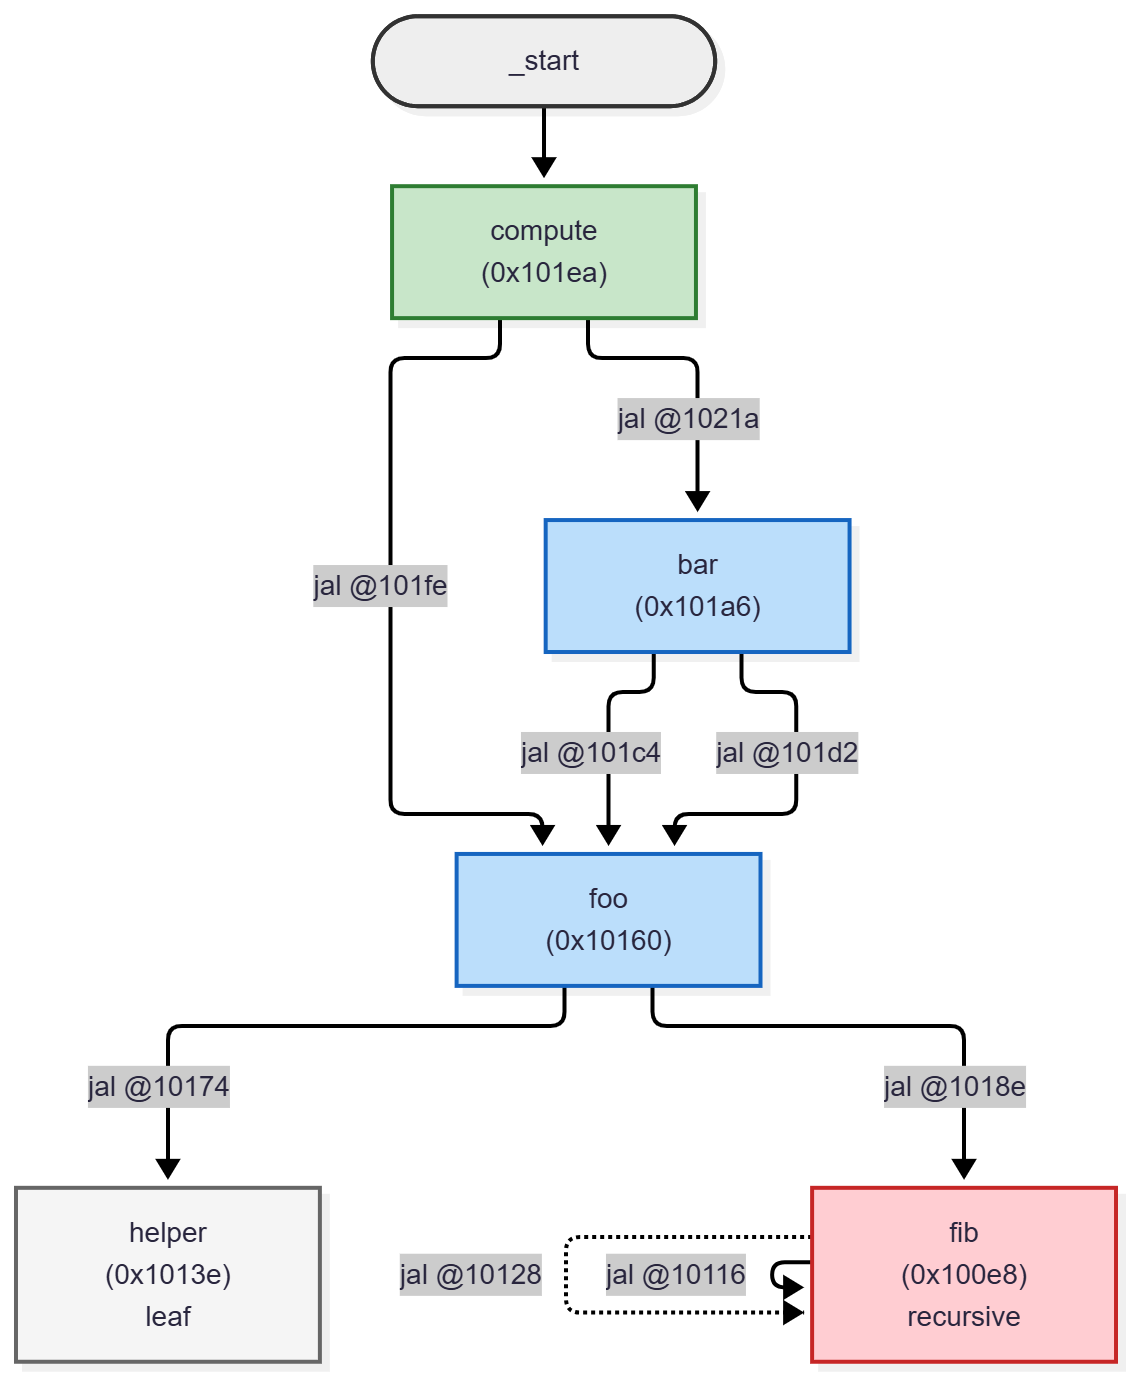
\includegraphics[width=0.7\textwidth]{figures/warmup_callgraph.png}

\caption{Warm-up call graph recovered from \texttt{warmup/build/challenge}.}
\label{fig:warmup}
\end{figure}

The graph can also be expressed in Mermaid:

\begin{lstlisting}[language=Mermaid,caption={Mermaid source for the warm-up call graph.}]
flowchart TD
    start[_start] --> compute
    compute -->|"jal @101fe"| foo
    compute -->|"jal @1021a"| bar
    foo -->|"jal @10174"| helper
    foo -->|"jal @1018e"| fib
    bar -->|"jal @101c4"| foo
    bar -->|"jal @101d2 (2nd call)"| foo
    fib -->|"jal @10116"| fib
    fib -.->|"jal @10128 (2nd call)"| fib
\end{lstlisting}

\subsection{Justification}

Starting from \texttt{compute} (\texttt{0x101ea}), its disassembly contains two \texttt{jal} instructions --- at \texttt{0x101fe} targeting \texttt{foo} (\texttt{0x10160}) and at \texttt{0x1021a} targeting \texttt{bar} (\texttt{0x101a6}) --- giving the first two graph edges. \texttt{foo}'s disassembly then shows \texttt{jal} calls to \texttt{helper} (\texttt{0x1013e}, at \texttt{0x10174}) and \texttt{fib} (\texttt{0x100e8}, at \texttt{0x1018e}); \texttt{bar}'s disassembly shows two \texttt{jal} calls, both to \texttt{foo} (at \texttt{0x101c4} and \texttt{0x101d2}). \texttt{helper} contains no further \texttt{jal} instructions, so it is a leaf; \texttt{fib} contains two \texttt{jal} instructions, both at \texttt{0x10116} and \texttt{0x10128}, both targeting \texttt{fib} itself (\texttt{0x100e8}) --- proving it is recursive. Since \texttt{foo} is a \texttt{jal} target inside both \texttt{compute}'s and \texttt{bar}'s disassembly, it is the function called from two different places.

% ============================================================
\section{Runbook}
% ============================================================

This runbook lets a new team member reproduce all three configurations from a clean checkout on a fresh Ubuntu 22.04/24.04 machine (native or WSL2). Every command below has been run and verified by the team.

\subsection{Prerequisites}

\begin{itemize}[leftmargin=*]
\item Ubuntu 22.04/24.04 LTS (native or WSL2)
\item Internet connection ($\sim$500\,MB for model checkpoints)
\item 3\,GB free disk space
\item \texttt{curl} (used by \texttt{fetch-models.sh})
\item A user account with \texttt{sudo} privileges
\end{itemize}

\subsection{Step 1: System Tools}

\begin{lstlisting}[language=bash]
sudo apt update
sudo apt install -y git build-essential gdb-multiarch qemu-system-misc \
  gcc-riscv64-linux-gnu binutils-riscv64-linux-gnu \
  binutils-riscv64-unknown-elf
\end{lstlisting}

\textbf{Expected:} each package installs without error. \\
\textbf{Verify:}
\begin{lstlisting}[language=bash]
qemu-system-riscv64 --version
riscv64-linux-gnu-objdump --version
riscv64-unknown-elf-objdump --version
gdb-multiarch --version
\end{lstlisting}
All four should print version info.

\subsection{Step 2: Clone Repository}

\begin{lstlisting}[language=bash]
cd ~
mkdir -p projects
cd projects
git clone https://github.com/Moorani/xv6-distributed-inference.git Milestone-1-
cd Milestone-1-
chmod +x *.sh
\end{lstlisting}

\textbf{Expected:} a new directory \texttt{Milestone-1-} containing the repository, with the shell scripts marked executable.

\subsection{Step 3: Python Tools}

\begin{lstlisting}[language=bash]
sudo apt install -y python3-venv python3-pip curl
python3 -m venv .venv
source .venv/bin/activate
pip install scapy pytest coloredlogs
\end{lstlisting}

\textbf{Important:} the prompt must start with \texttt{(.venv)} after activation. Activate \texttt{.venv} in \emph{every new terminal} before running any Python or pytest command.

\subsection{Step 4: Model Checkpoints}

\begin{lstlisting}[language=bash]
./fetch-models.sh
./fetch-models.sh --check
\end{lstlisting}

\textbf{Expected:} three files downloaded into \texttt{server/models/}:
\begin{center}
\begin{tabular}{llr}
\toprule
Id & File & Size (bytes) \\
\midrule
1 & stories15M.bin & 60,816,028 \\
2 & tokenizer.bin   & 433,869 \\
3 & stories110M.bin & 438,381,596 \\
\bottomrule
\end{tabular}
\end{center}
Verify with \texttt{ls -la server/models/}. The \texttt{--check} flag re-verifies without downloading.

\textbf{Note:} the first run of \texttt{llama} will sit at ``Fetching from server\ldots'' for about 75--110 seconds while it downloads 60\,MB of weights over emulated UDP. This is normal and only happens once per boot session.

\subsection{Configuration 1: Single Node}

\textbf{Terminal 1} --- start the weight server (leave running):
\begin{lstlisting}[language=bash]
cd ~/projects/Milestone-1-
source .venv/bin/activate
python server/server.py
\end{lstlisting}

\textbf{Terminal 2} --- boot the node and run inference:
\begin{lstlisting}[language=bash]
cd ~/projects/Milestone-1-
source .venv/bin/activate
XV6_CPUS=1 ./boot.sh
# Inside the xv6 shell:
llama -t 0 -n 32 -i "Once upon a time"
\end{lstlisting}

\textbf{Expected:} after the initial weight fetch, the model prints coherent generated text followed by a performance profile. To exit QEMU: press \texttt{Ctrl-a}, release, then \texttt{x}.

\subsection{Configuration 2: Multi-Node Ring}

\begin{lstlisting}[language=bash]
cd ~/projects/Milestone-1-
pkill -f qemu-system-riscv64
pkill -f mcast_switch.py
source .venv/bin/activate
python3 server/distinf_sim.py --workers 2 --model 1 --steps 32 \
  --prompt "Once upon a time" --smp 2 --shard-timeout 1800
\end{lstlisting}

For 3 workers, change \texttt{--workers 3}. For the larger model, change \texttt{--model 3} (up to 12 workers).

\textbf{Expected:} the simulator boots all nodes, prints worker registration, shard fetch, generation, and a \texttt{PASS} result with the generated text.

\subsubsection*{Two important gotchas (both discovered during bring-up)}

\begin{enumerate}[leftmargin=*]
\item \textbf{You \emph{must} activate \texttt{.venv} before running \texttt{distinf\_sim.py}.} The simulator launches its helper process \texttt{server/mcast\_switch.py} with whatever Python interpreter invoked the main script. If \texttt{.venv} is not active, system Python is missing \texttt{coloredlogs} and \texttt{mcast\_switch.py} crashes silently. The symptom is an ARP-timeout in the master log (\texttt{arp\_lookup: resolution timed out for 0xa000001}) with no other error message --- it looks like a network problem but is actually a missing Python package.

\item \textbf{Use \texttt{--shard-timeout 1800}.} The default 900-second shard-fetch timeout is too short on consumer hardware: the 35\,MB embedding fetch for each worker can take longer than 900\,s under contention. If the default is used, the simulator kills the QEMU nodes on timeout and reports \texttt{FAIL -- never assigned layers within 900s}.
\end{enumerate}

\subsection{Configuration 3: Weight-Fetch Path}

\textbf{Terminal 1} --- start the weight server (leave running):
\begin{lstlisting}[language=bash]
cd ~/projects/Milestone-1-
source .venv/bin/activate
python server/server.py
\end{lstlisting}

\textbf{Terminal 2} --- boot the node and run \texttt{testftp}:
\begin{lstlisting}[language=bash]
cd ~/projects/Milestone-1-
source .venv/bin/activate
./boot.sh
# Inside the xv6 shell:
testftp
\end{lstlisting}

\textbf{Expected:} the program fetches the tokenizer and weights and prints the number of bytes transferred for each, with SHA-256 checksums:
\begin{lstlisting}[language=,basicstyle=\ttfamily\footnotesize]
PASS    Successfully fetched tokenizer: 433869 bytes
  Final SHA-256: 50a52ef8...
PASS    Successfully fetched weights: 60816028 bytes
  Final SHA-256: cd590644...
PASS   LLM file transfer test completed
\end{lstlisting}

% ============================================================
\section{Architecture Map}
% ============================================================

The eight subsystems are mapped below. Rows 1 and 8 live in the kernel, whose \texttt{.c} source was withheld; they are mapped from the binary via \texttt{nm} and \texttt{objdump}. Rows 2--7 are user-space and are mapped from source.

\begin{longtable}{@{}p{0.4cm}p{3.1cm}p{3.2cm}p{3.6cm}p{4.5cm}@{}}
\toprule
\textbf{\#} & \textbf{Subsystem} & \textbf{Entry point} & \textbf{Location} & \textbf{Standard / Responsibility} \\
\midrule
\endfirsthead
\toprule
\textbf{\#} & \textbf{Subsystem} & \textbf{Entry point} & \textbf{Location} & \textbf{Standard / Responsibility} \\
\midrule
\endhead
1 & Network stack & \texttt{net\_rx} & \texttt{kernel/net.c}, symbol at \texttt{0x800099c6} & RFC 791, RFC 1122. Ethernet frame dispatch to ARP/IP by EtherType at frame offset 12--13. Supporting: \texttt{arp\_lookup} at \texttt{0x80007bd8}. \\
2 & Remote procedure call & \texttt{rpc\_init(uint16 local\_port)} & \texttt{user/rpc.c:138}, \texttt{user/rpc.h:235} & RFC 5531 \S9 (message format), \S5 (UDP timeout/retransmit), \S8.3 (program-number block \texttt{0x20000001}). Sun-RPC call/reply. \\
3 & Data serialisation & \texttt{xdrmem\_create(XDR*, char*, u\_int, enum xdr\_op)} & \texttt{user/xdr.c:143}, \texttt{user/xdr.h:77} & RFC 4506. Memory-backed XDR stream creation for encode/decode. \\
4 & Discovery and registration & \texttt{discovery\_register(const rpc\_addr\_t*, worker\_info\_t*, set\_neighbor\_t*)} & \texttt{user/discovery.c:288}, \texttt{user/discovery.h:161} & RFC 2104 / FIPS 198-1 (HMAC-SHA256 keyed MAC). Registration wire message \texttt{PROC\_AUTH\_HELLO}. State machine: \texttt{WORKER\_PENDING}, \texttt{ACTIVE}, \texttt{SUSPECTED}, \texttt{EXPIRED}. \\
5 & Ring driver / shard logic & \texttt{main(int argc, char *argv[])}; per-hop \texttt{worker\_infer} & \texttt{user/distinf.c:1551}; \texttt{worker\_infer} at \texttt{distinf.c:6000}; \texttt{shard\_load} at \texttt{user/shard.c:103} & RFC 4506 (XDR, new payloads); RFC 791 (hop size deliberately above 1500-byte MTU). Drives the master/worker ring and per-hop forwarding. \\
6 & Transformer kernels & \texttt{forward(Transformer*, int token, int pos)} & \texttt{user/llama\_core.c:742}, \texttt{user/llama\_core.h:247} & Port of Karthik/Andrej Karpathy's \texttt{llama2.c}. Full forward pass shared by single-node and sharded workers. \\
7 & Weight-fetch client & \texttt{fetch\_model\_weights(int *size\_out)} built on \texttt{llm\_fetch\_file} & \texttt{user/ftpclient.c}, \texttt{user/ftpclient.h:84,197} & Self-defined RFTP protocol: \texttt{META\_REQ}, \texttt{DATA\_RANGE\_REQ}, \texttt{RETRANS\_REQ}. SHA-256 integrity check. \\
8 & Kernel hardening set & \texttt{stackguard\_init}; \texttt{random\_init}, \texttt{capable}, \texttt{sys\_getrlimit}/\texttt{sys\_setrlimit}, \texttt{mappages}/\texttt{flags2perm} & \texttt{kernel/stackguard.c} at \texttt{0x80001e64}; \texttt{random\_init} at \texttt{0x80002000}; \texttt{random\_add} at \texttt{0x80001e94}; \texttt{capable} at \texttt{0x800069d6}; \texttt{sys\_getentropy} at \texttt{0x80001b46}; \texttt{sys\_getrlimit} at \texttt{0x80001a44}; \texttt{sys\_setrlimit} at \texttt{0x80001982}; \texttt{rlimit\_as\_ok} at \texttt{0x8000693a}; \texttt{mappages} at \texttt{0x8000051c}; \texttt{flags2perm} at \texttt{0x80004884} & POSIX.1-2017 (\texttt{getrlimit}/\texttt{setrlimit}); POSIX.1e capability model. Stack canary (\texttt{\_\_stack\_chk\_guard}/\texttt{\_\_stack\_chk\_fail}), entropy source, capability checks, resource limits, W\^{}X enforcement. \\
\bottomrule
\caption{Architecture map of the eight subsystems.}
\end{longtable}

\textbf{Notes from disassembly:}
\begin{itemize}[leftmargin=*]
\item \texttt{net\_rx} reads the two EtherType bytes at frame offset 12--13, compares against byte-swapped constants \texttt{1544} (\texttt{0x0608} = byte-swapped \texttt{0x0806}, ARP) and \texttt{8} (\texttt{0x0008} = byte-swapped \texttt{0x0800}, IP), and calls \texttt{arp\_rx} (\texttt{0x800094e8}) or \texttt{ip\_rx} (\texttt{0x80008d9a}) respectively. Anything else is dropped via \texttt{kfree}.
\item \texttt{stackguard\_init} calls \texttt{rand64()} (\texttt{0x80001f3c}) and stores the result directly into the global \texttt{\_\_stack\_chk\_guard}. The entropy source (row 8's \texttt{random\_init}/\texttt{random\_add}) and the stack-canary mechanism are the same subsystem, seeded once at boot.
\end{itemize}

% ============================================================
\section{Kernel Trace}
% ============================================================

The kernel ships as a compiled binary with a symbol table but no \texttt{.c} source (Section~2.9 of the handout). We traced two entry-point functions: one by static disassembly (\texttt{net\_rx}), one under the debugger (\texttt{sys\_exec}). Both are presented here as evidence for the Reverse-Engineering Workflow rubric item.

\subsection{Static trace: \texttt{net\_rx}}

\begin{lstlisting}[language=bash]
riscv64-unknown-elf-objdump -d --disassemble=net_rx kernel/kernel
\end{lstlisting}

The annotated disassembly (extract):

\begin{lstlisting}[language=,basicstyle=\ttfamily\footnotesize]
800099c6 <net_rx>:
  ...
  lhu   a5,12(a5)        # read EtherType at frame offset 12
  ...
  li    a4,1544          # 0x0608 (byte-swapped 0x0806 = ARP)
  beq   a5,a4,.Larp
  li    a4,8             # 0x0008 (byte-swapped 0x0800 = IP)
  beq   a5,a4,.Lip
  ...                    # else: kfree(buf)
.Larp:
  jal   800094e8 <arp_rx>
.Lip:
  jal   80008d9a <ip_rx>
\end{lstlisting}

\texttt{net\_rx} is the driver-to-kernel handoff: the e1000 driver's receive path calls it for every incoming frame, and it dispatches by EtherType to the ARP or IP handler. Frames of any other type are freed.

\subsection{Dynamic trace: \texttt{sys\_exec} under gdb}

Terminal~1 (kernel halted, gdb stub on port 26000):
\begin{lstlisting}[language=bash]
cd ~/projects/Milestone-1-
pkill -f qemu-system-riscv64
./boot-gdb.sh
\end{lstlisting}

Terminal~2 (attach gdb):
\begin{lstlisting}[language=bash]
cd ~/projects/Milestone-1-/xv6-riscv
gdb-multiarch kernel/kernel
\end{lstlisting}

Inside gdb:
\begin{lstlisting}[language=,basicstyle=\ttfamily\footnotesize]
(gdb) target remote localhost:26000
Remote debugging using localhost:26000
0x0000000000001000 in ?? ()
(gdb) break sys_exec
Breakpoint 1 at 0x80005856
(gdb) continue
Continuing.

Breakpoint 1, 0x0000000080005856 in sys_exec ()
(gdb) backtrace
#0  0x0000000080005856 in sys_exec ()
#1  0x00000000800014dc in syscall ()
#2  0x0000000080001224 in usertrap ()
#3  0x0000003ffffff124 in ?? ()
(gdb) info registers a0 a1 a2
a0             0x1      1
a1             0x3fffffbdf8     274877890040
a2             0x1      1
(gdb) info registers sp
sp             0x3fffffbdf0     0x3fffffbdf0
(gdb) stepi
0x000000008000142c in argaddr ()
(gdb) stepi
0x000000008000142e in argaddr ()
(gdb) continue
Continuing.
^C
Program received signal SIGINT, Interrupt.
0x0000000080006bda in scheduler ()
(gdb) quit
\end{lstlisting}

\textbf{Interpretation.} \texttt{sys\_exec} is reached via the standard xv6 syscall dispatch path: a user-mode \texttt{ecall} traps into \texttt{usertrap} (\texttt{0x80001224}), which calls \texttt{syscall} (\texttt{0x800014dc}), which dispatches to \texttt{sys\_exec} (\texttt{0x80005856}). The disassembly of \texttt{sys\_exec} at \texttt{0x80005850} shows the sequence:

\begin{lstlisting}[language=,basicstyle=\ttfamily\footnotesize]
80005850: addi a1,s0,-456    # a1 = destination stack slot
80005854: li   a0,1          # a0 = 1 (fetch argv, the 2nd exec argument)
80005856: jal  argaddr        # <- breakpoint lands here
\end{lstlisting}

So the captured \texttt{a0=1} is the argument index passed to \texttt{argaddr}, and \texttt{a1=0x3fffffbdf8} is the kernel-stack destination where the fetched user pointer is written. That address is a kernel-stack address (below \texttt{TRAMPOLINE}, near the top of the process's kernel virtual address space), not a user-space pointer.

The observed \texttt{sp=0x3fffffbdf0} is consistent with \texttt{memlayout.h}'s formula \texttt{KSTACK(p) = TRAMPOLINE - (p+1)*2*PGSIZE}, where \texttt{TRAMPOLINE = MAXVA - PGSIZE}. Each process's kernel stack occupies a \texttt{2*PGSIZE} slot beneath the trampoline, separated from neighbouring stacks by unmapped guard pages, so a stack overflow faults rather than corrupting the next process's stack. This is the same high-address region reserved at the top of every process's kernel virtual address space.

The two \texttt{stepi} commands landing inside \texttt{argaddr} (\texttt{0x8000142c}) confirm that \texttt{sys\_exec}'s first action is to call the standard argument-fetching helper for the \texttt{argv} pointer.

% ============================================================
\section{Figures F1--F7}
% ============================================================

All seven figures are written in Mermaid. The source for each is committed under \texttt{docs/figures/}; the rendered images appear here, numbered, captioned, and referred to in the text.

\subsection{F1: System Architecture}

\begin{figure}[H]
\centering
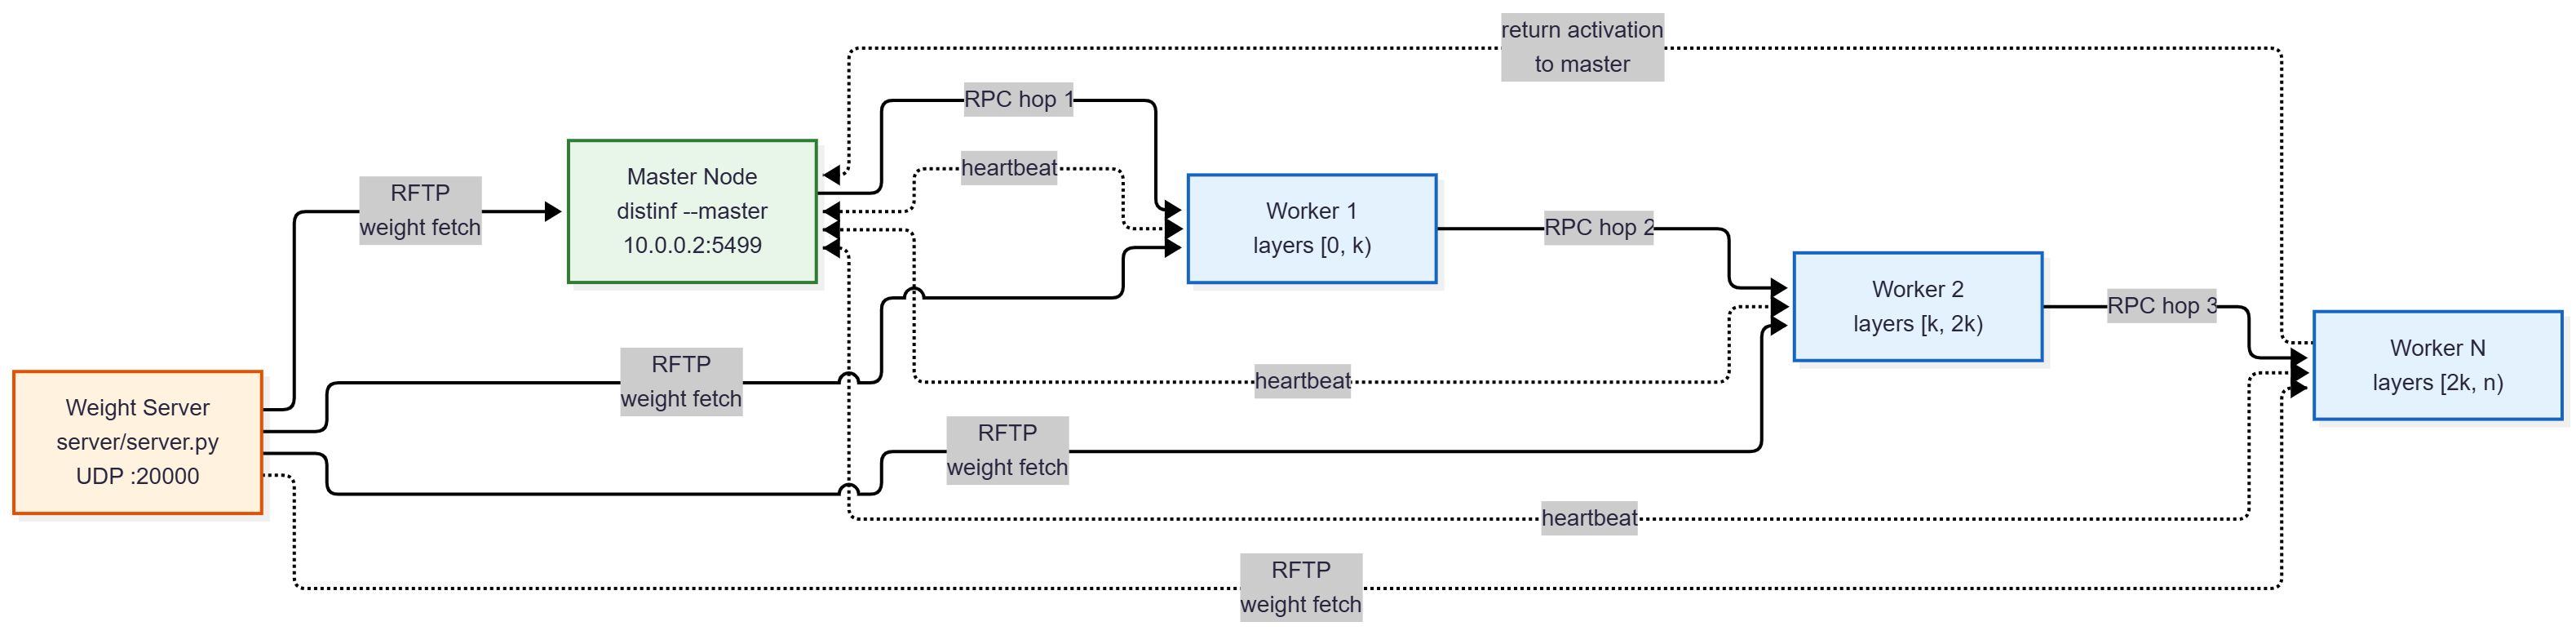
\includegraphics[width=\textwidth]{figures/F1.png}
\caption{System architecture: weight server, master, $N$ workers, the ring, and the transport between them.}
\label{fig:F1}
\end{figure}

\begin{lstlisting}[language=Mermaid,caption={F1 Mermaid source.}]
flowchart LR
    WS[Weight Server<br/>server/server.py<br/>UDP :20000] -->|RFTP| M
    M[Master Node<br/>distinf --master<br/>10.0.0.2:5499] -->|RPC hop 1| W1[Worker 1<br/>layers 0..k]
    W1 -->|RPC hop 2| W2[Worker 2<br/>layers k..2k]
    W2 -->|RPC hop 3| W3[Worker 3<br/>layers 2k..n]
    W3 -.->|return activation| M
    W1 <-.heartbeat.-> M
    W2 <-.heartbeat.-> M
    W3 <-.heartbeat.-> M
\end{lstlisting}

\subsection{F2: Wire Format}

\begin{figure}[H]
\centering
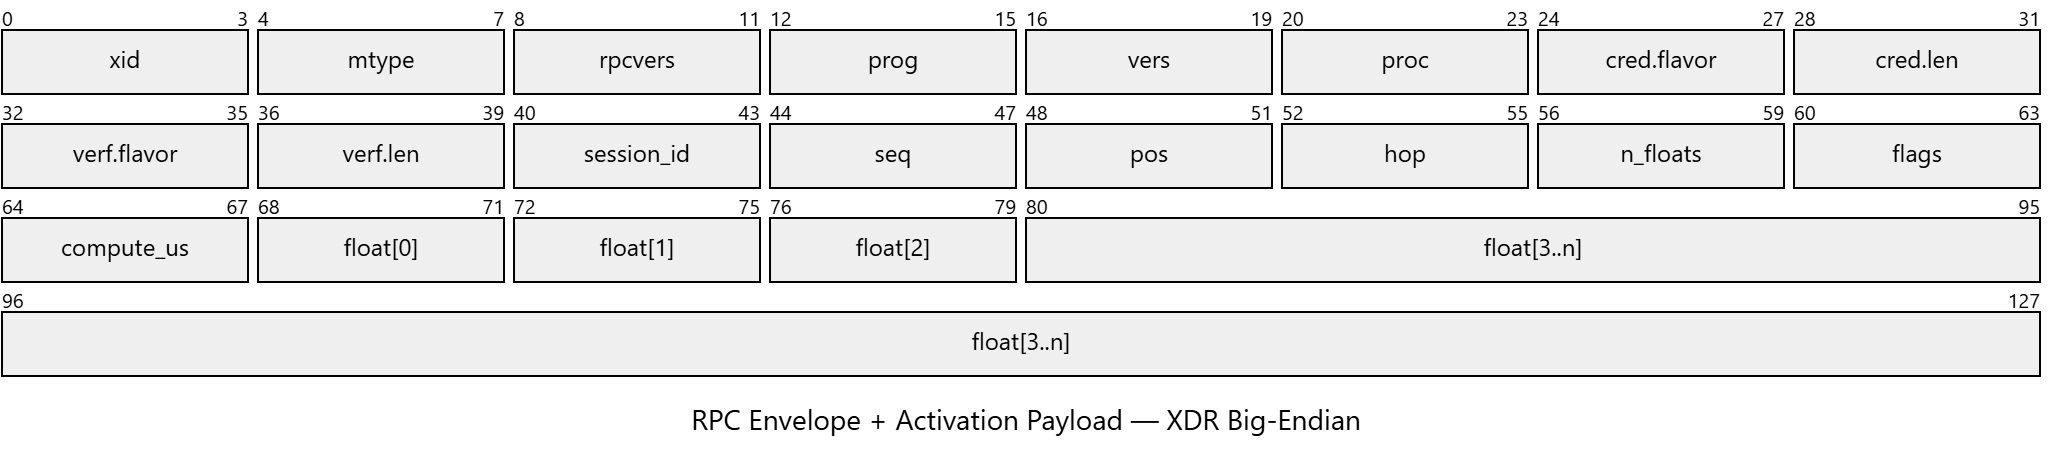
\includegraphics[width=\textwidth]{figures/F2.png}

\caption{RPC envelope and activation layout at byte level (7 header words + $n$\_floats $\times$ 4 bytes, XDR big-endian).}
\label{fig:F2}
\end{figure}

\begin{lstlisting}[language=Mermaid,caption={F2 Mermaid source.}]
packet-beta
0-3: "xid (4 bytes) — transaction ID"
4-7: "mtype (4 bytes) — MSG_CALL (0) or MSG_REPLY (1)"
8-11: "rpcvers (4 bytes) — RPC_VERSION (2)"
12-15: "prog (4 bytes) — INFERENCE_PROG (0x20000001)"
16-19: "vers (4 bytes) — INFERENCE_VERS (1)"
20-23: "proc (4 bytes) — procedure number (0-10)"
24-27: "cred.flavor (4 bytes) — AUTH_NONE (0)"
28-31: "cred.body_len (4 bytes) — 0"
32-35: "verf.flavor (4 bytes) — AUTH_NONE (0)"
36-39: "verf.body_len (4 bytes) — 0"
40-43: "payload[0..3] — activation header word 0 (session_id)"
44-47: "payload[4..7] — word 1 (seq)"
48-51: "payload[8..11] — word 2 (pos)"
52-55: "payload[12..15] — word 3 (hop)"
56-59: "payload[16..19] — word 4 (n_floats)"
60-63: "payload[20..23] — word 5 (flags)"
64-67: "payload[24..27] — word 6 (compute_us)"
68-71: "payload[28..31] — activation float 0 (XDR big-endian)"
72-75: "payload[32..35] — activation float 1"
76-79: "payload[36..39] — activation float 2"
80-383: "... up to n_floats x 4 bytes"
\end{lstlisting}

\subsection{F3: Worker Lifecycle}

\begin{figure}[H]
\centering
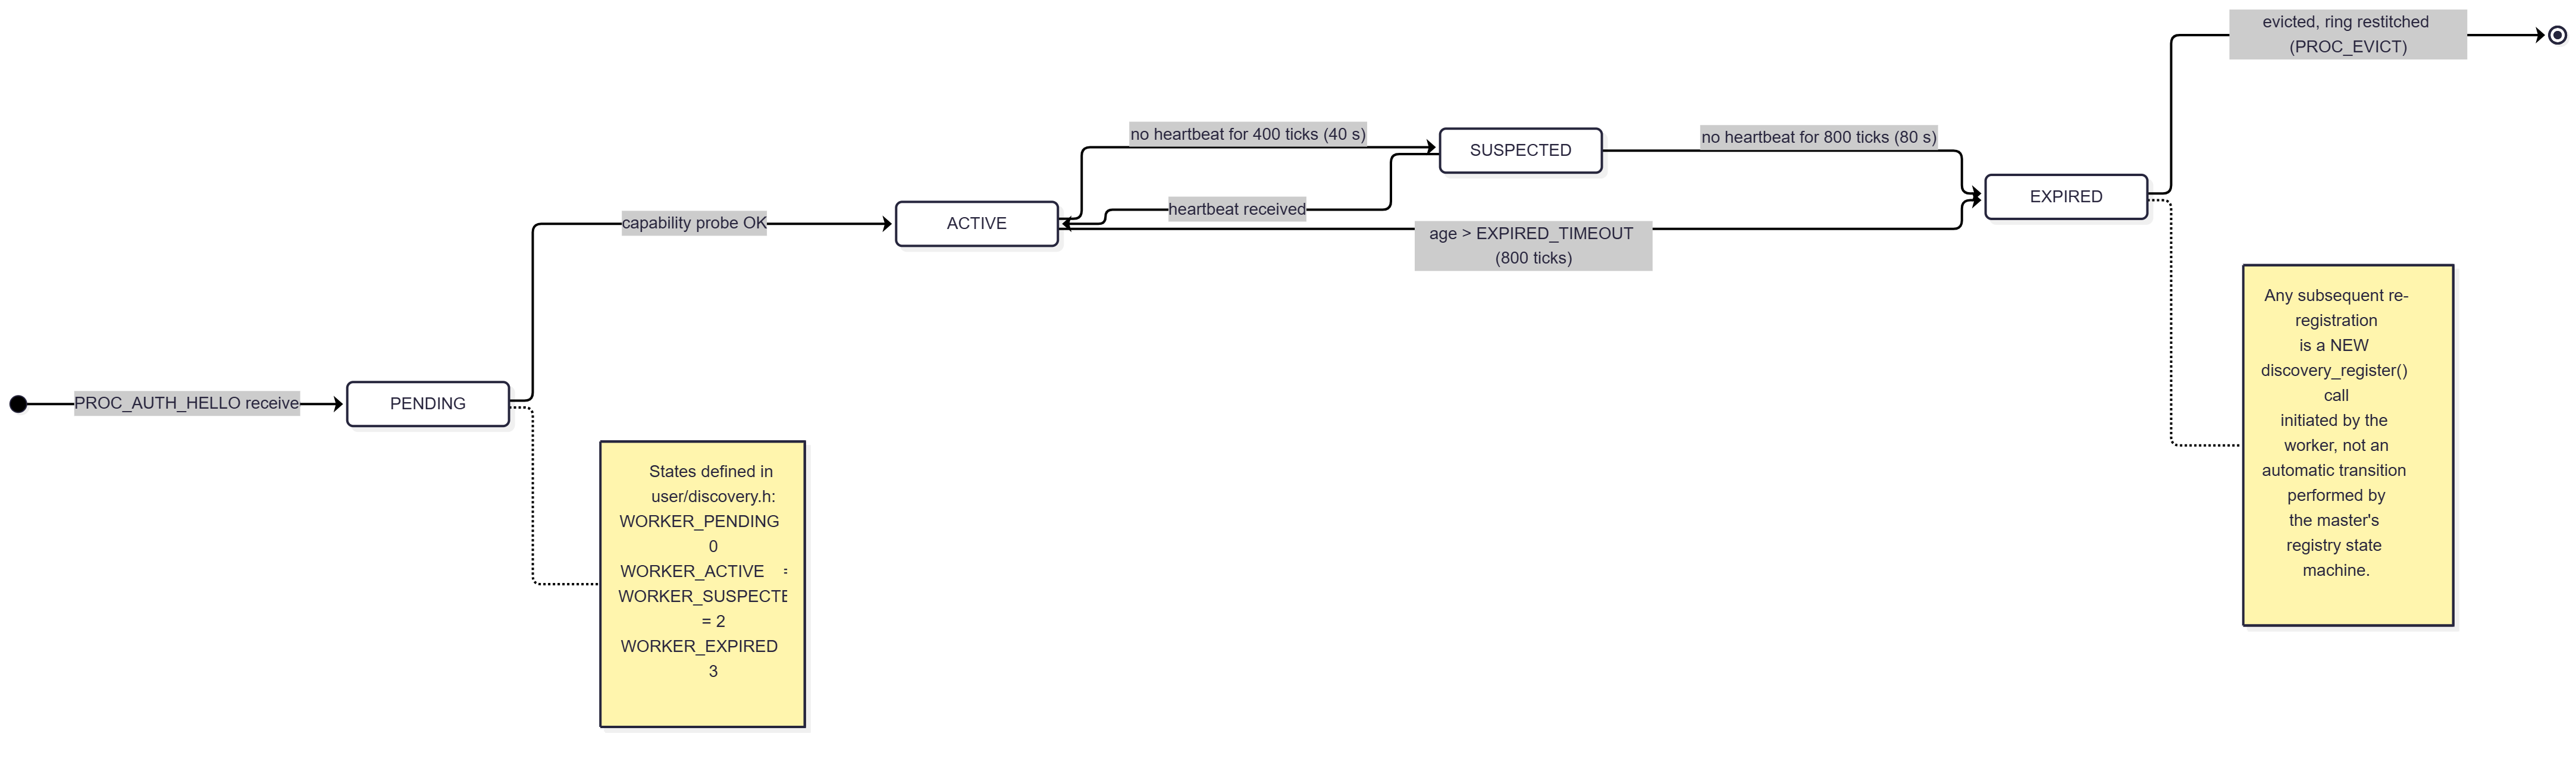
\includegraphics[width=0.75\textwidth]{figures/F3.png}

\caption{Worker lifecycle state machine as implemented in code.}
\label{fig:F3}
\end{figure}

\begin{lstlisting}[language=Mermaid,caption={F3 Mermaid source.}]
stateDiagram-v2
    [*] --> PENDING : PROC_AUTH_HELLO received
    PENDING --> ACTIVE : capability probe OK
    ACTIVE --> SUSPECTED : HEARTBEAT_INTERVAL_TICKS(200) x HEARTBEAT_MISS_SUSPECTED(2) = 400 ticks (40 s at 10 Hz)
    SUSPECTED --> ACTIVE : heartbeat received
    SUSPECTED --> EXPIRED : HEARTBEAT_INTERVAL_TICKS(200) x HEARTBEAT_MISS_EXPIRED(4) = 800 ticks (80 s)
    ACTIVE --> EXPIRED : age > EXPIRED_TIMEOUT (800 ticks)
    EXPIRED --> [*] : evicted, ring restitched (PROC_EVICT)
    note right of EXPIRED
      Any subsequent re-registration
      is a new discovery_register() call
      initiated by the worker.
    end note
\end{lstlisting}

\paragraph{Divergence from \texttt{diagrams/state\_diagram.png}.}
The repository's hand-drawn diagram shows three divergences from the code. (1)~It shows \texttt{PENDING ---timeout$\to$ unregistered}, whereas the code ages a \texttt{PENDING} worker through \texttt{SUSPECTED} then \texttt{EXPIRED}. (2)~It has an ``unregistered'' state that does not exist in the code: \texttt{discovery.h} defines exactly four states (\texttt{WORKER\_PENDING=0}, \texttt{WORKER\_ACTIVE=1}, \texttt{WORKER\_SUSPECTED=2}, \texttt{WORKER\_EXPIRED=3}), and \texttt{discovery\_register()} creates a \texttt{PENDING} entry directly on receipt of \texttt{PROC\_AUTH\_HELLO} --- there is no separate ``unregistered'' holding state a worker passes through first. (3)~The diagram labels the \texttt{ACTIVE$\to$SUSPECTED} and \texttt{SUSPECTED$\to$EXPIRED} transitions only ``heartbeat timeout'' / ``final heartbeat timeout'' with no timing; the code's thresholds are concrete and tick-based: \texttt{SUSPECTED\_TIMEOUT = 200 $\times$ 2 = 400 ticks (40\,s at 10\,Hz)} and \texttt{EXPIRED\_TIMEOUT = 200 $\times$ 4 = 800 ticks (80\,s)}, and the code ages \emph{any} state directly to \texttt{EXPIRED} once age $>$ \texttt{EXPIRED\_TIMEOUT}, not only \texttt{PENDING}. The diagram also draws an automatic recovery arrow from ``worker expired'' back up to ``hello'', implying the master's state machine loops a worker back to re-registration on its own; in the code, \texttt{discovery\_expire\_workers()} only evicts the entry and restitches the ring (\texttt{PROC\_EVICT}) --- any subsequent registration is a brand-new, independent \texttt{discovery\_register()} call initiated by the worker, not a transition the master's registry state machine performs. The \texttt{PENDING$\to$ACTIVE} (on capability-probe success) and \texttt{SUSPECTED$\to$ACTIVE} (on heartbeat received) edges are the only parts of the hand-drawn diagram that are directionally correct.

\subsection{F4: Token Sequence}

\begin{figure}[H]
\centering
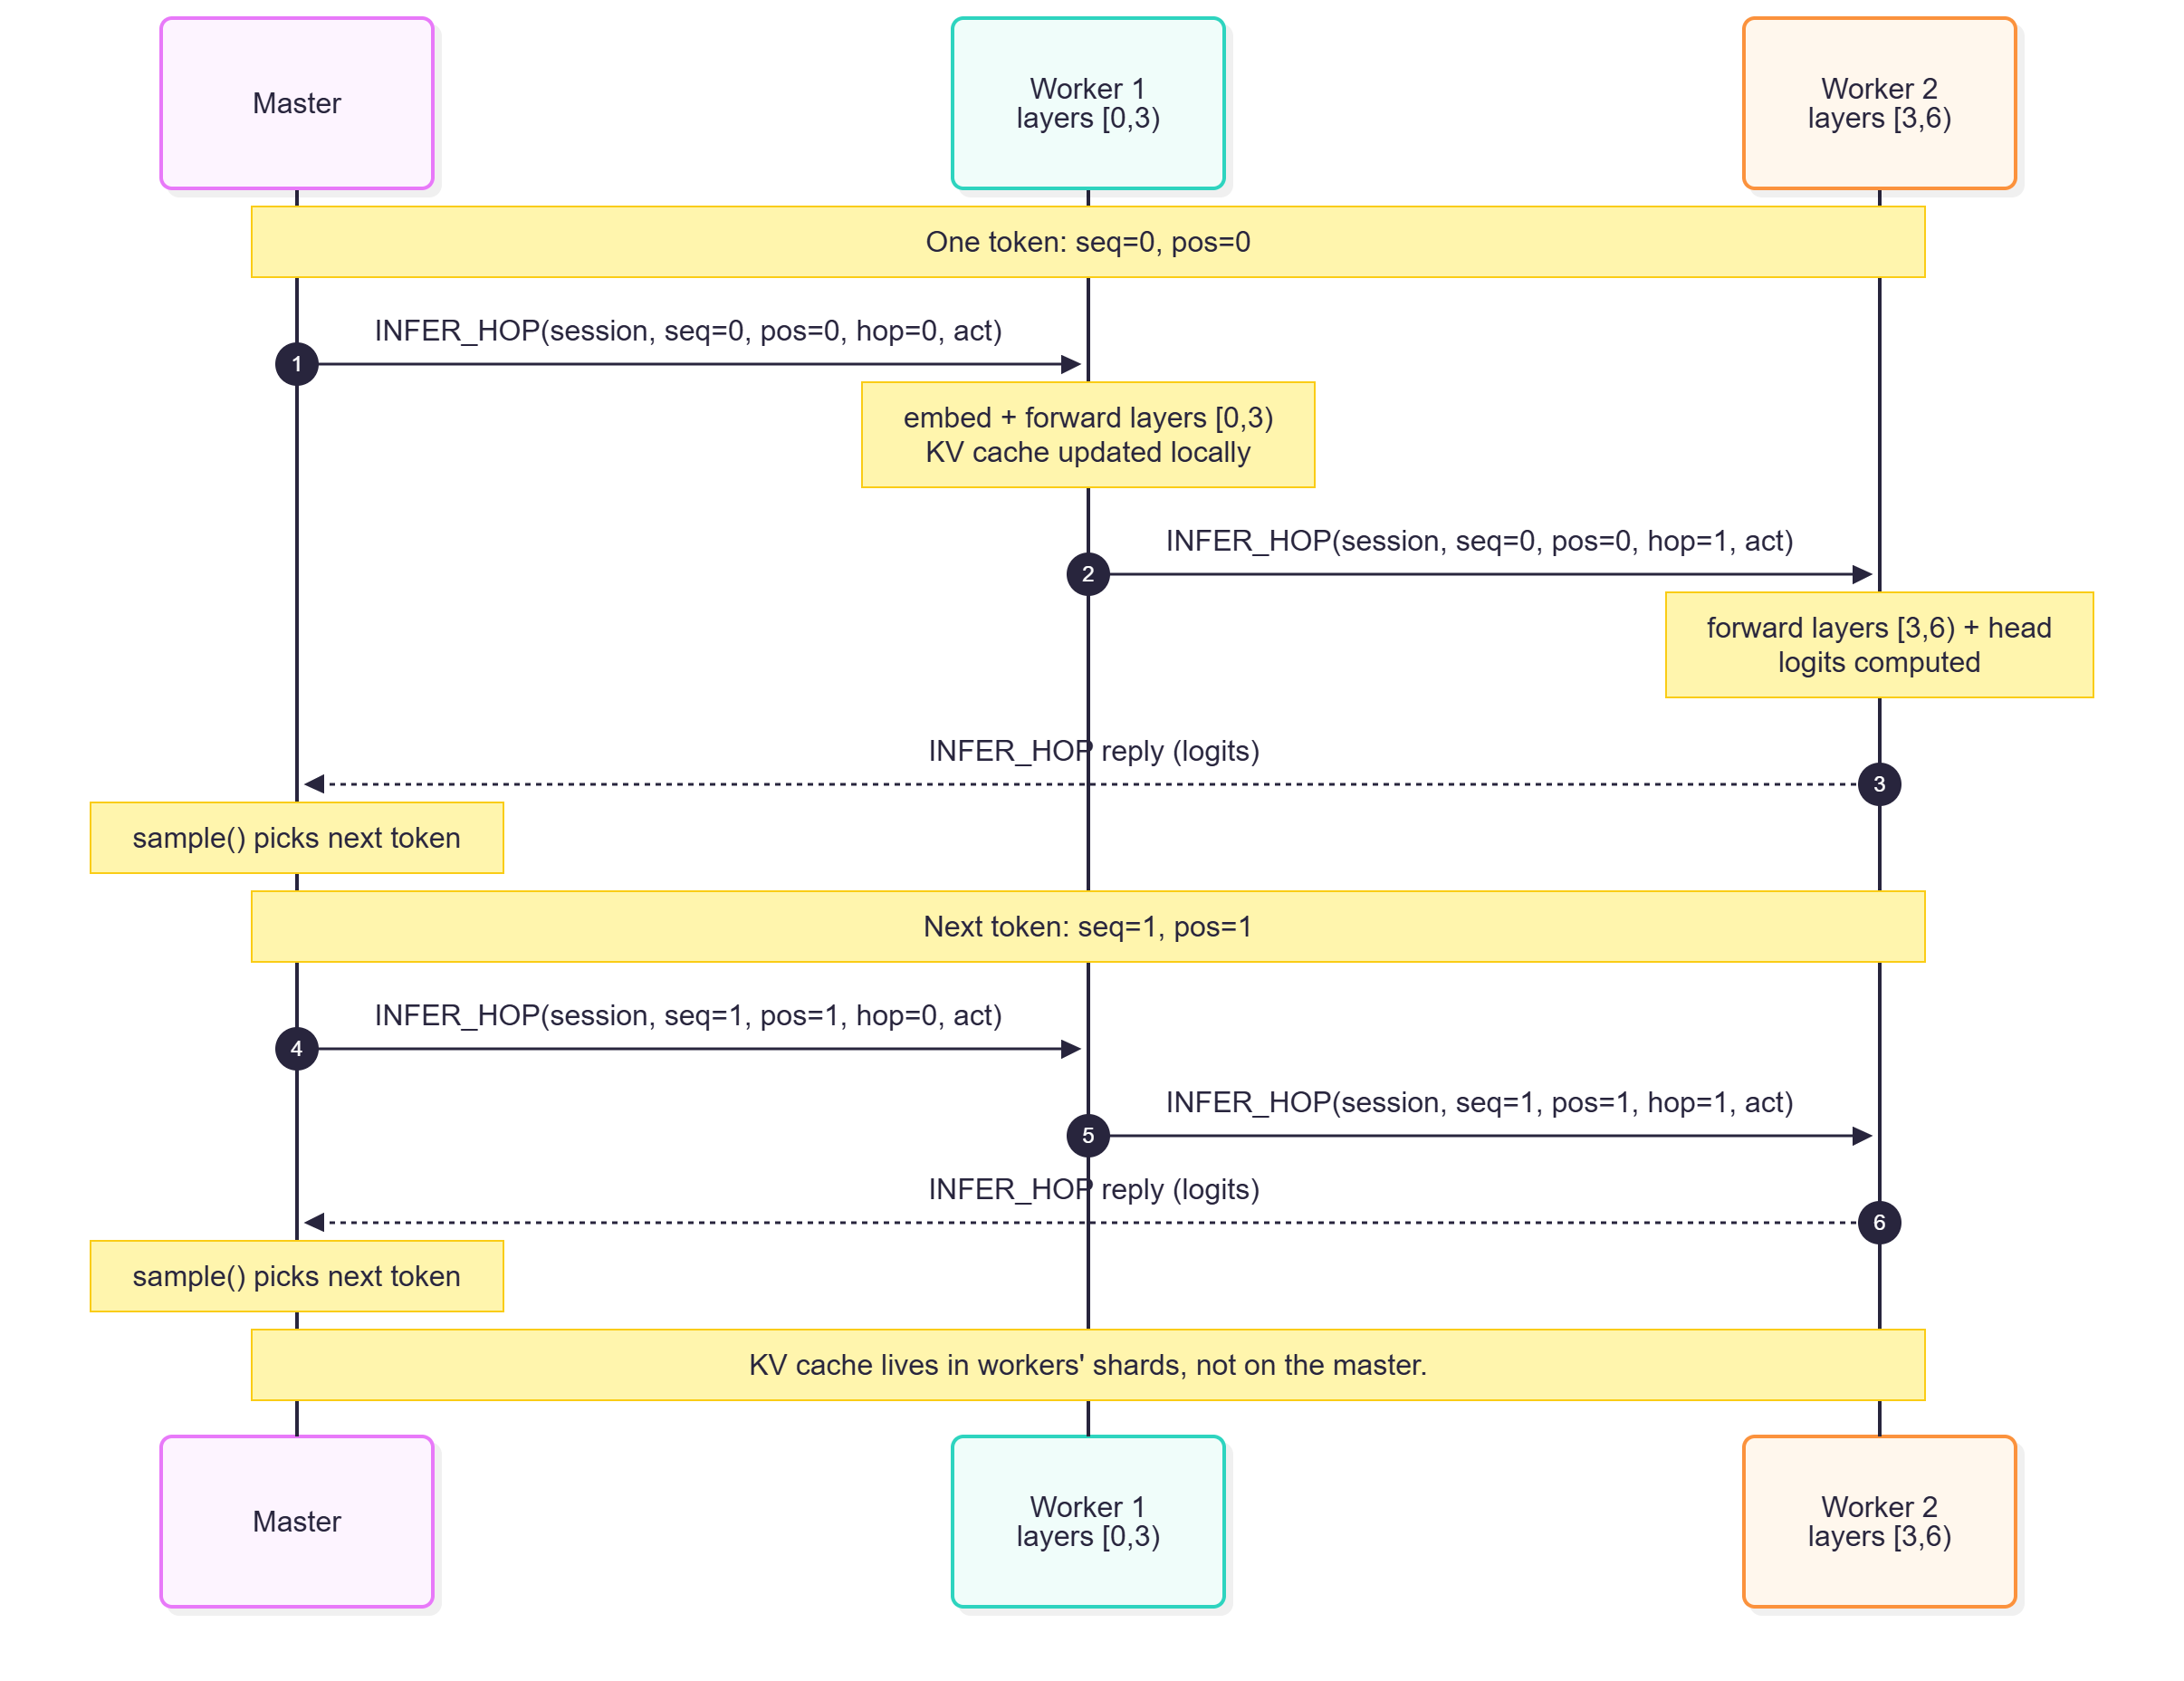
\includegraphics[width=\textwidth]{figures/F4.png}

\caption{One token from master through each worker and back. KV cache lives in the workers' shards, not on the master. Layers $[0,3)$ and $[3,6)$.}
\label{fig:F4}
\end{figure}

\begin{lstlisting}[language=Mermaid,caption={F4 Mermaid source.}]
sequenceDiagram
    participant M as Master
    participant W1 as Worker 1 [0,3)
    participant W2 as Worker 2 [3,6)
    M->>W1: INFER_HOP(session,seq=0,pos=0,hop=0,act)
    Note over W1: embed + layers [0,3)
    W1->>W2: INFER_HOP(session,seq=0,pos=0,hop=1,act)
    Note over W2: layers [3,6) + head
    W2-->>M: INFER_HOP reply (logits + sampled token)
    Note over M: sample() picks next token
    M->>W1: INFER_HOP(seq=1,pos=1,hop=0,...)
    W1->>W2: INFER_HOP(seq=1,pos=1,hop=1,...)
    W2-->>M: INFER_HOP reply
\end{lstlisting}

\subsection{F5: Inference Hot Path}

\begin{figure}[H]
\centering
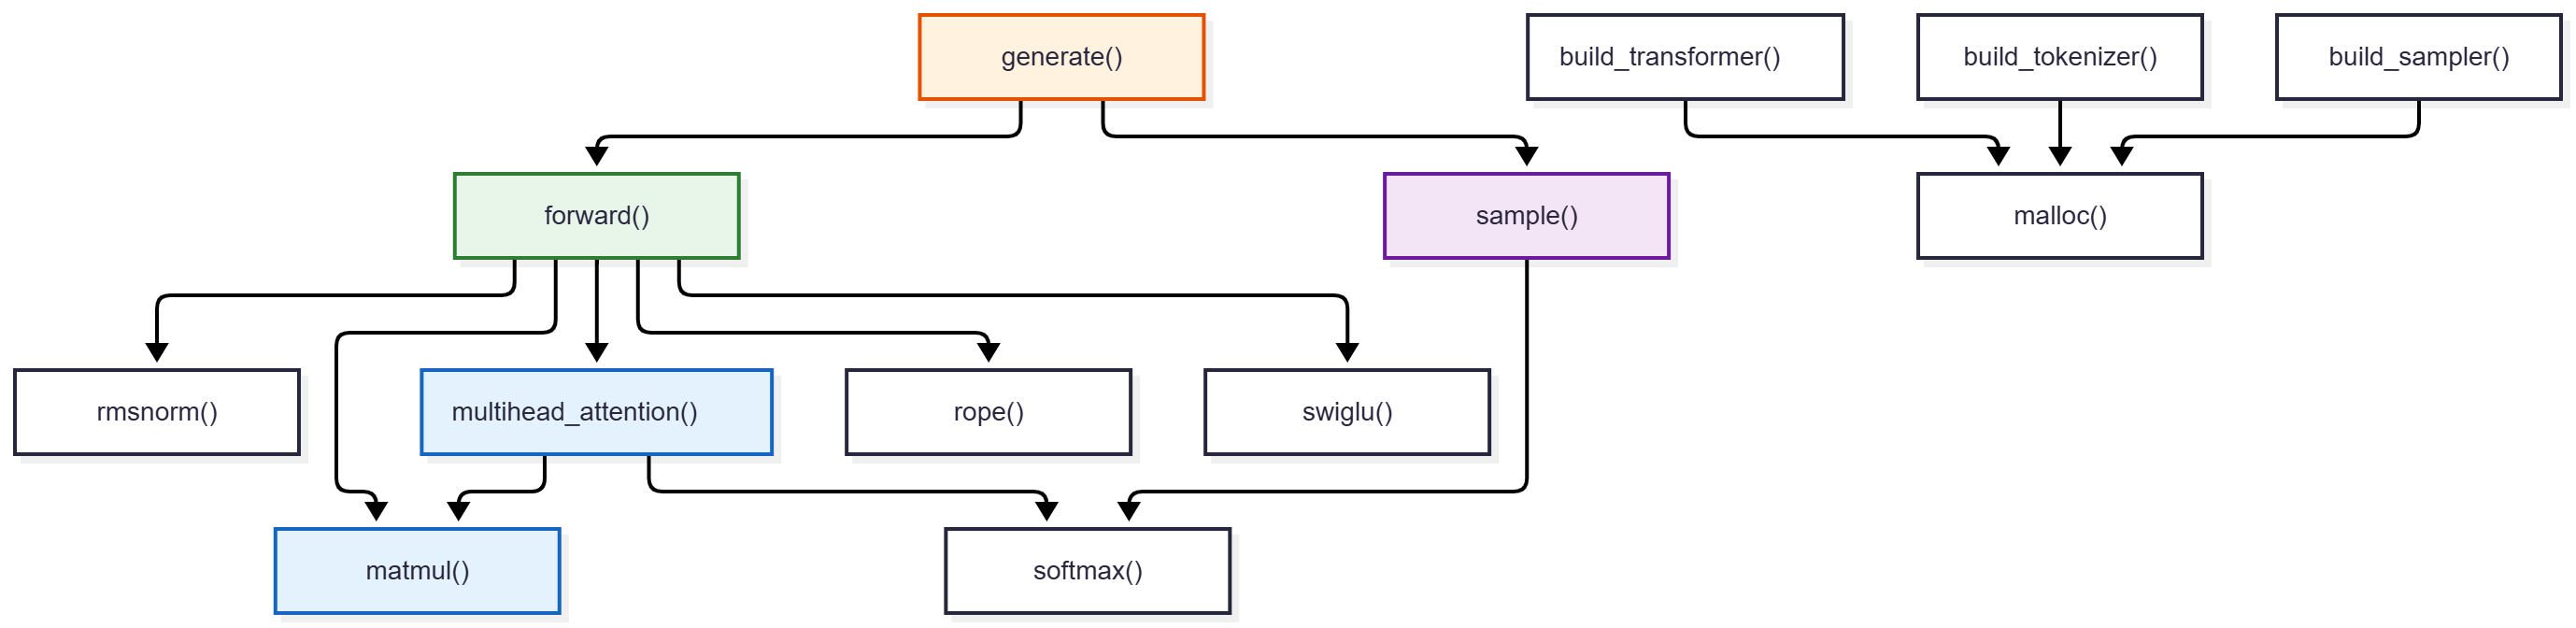
\includegraphics[width=0.85\textwidth]{figures/F5.png}

\caption{Call graph through \texttt{user/llama\_core.c}. \texttt{sample()} is called by \texttt{generate()}, not by \texttt{forward()}.}
\label{fig:F5}
\end{figure}

\begin{lstlisting}[language=Mermaid,caption={F5 Mermaid source (style follows \texttt{syscall\_dependency\_diagram.md}).}]
flowchart TD
    generate[generate] --> forward[forward]
    generate --> sample[sample]
    forward --> rmsnorm[rmsnorm]
    forward --> matmul[matmul]
    forward --> multihead_attention[multihead\_attention]
    forward --> rope[rope]
    forward --> swiglu[swiglu]
    multihead_attention --> matmul
    multihead_attention --> softmax[softmax]
    rmsnorm --> rmsnorm_w[rmsnorm\_weights]
    sample --> softmax
    build_transformer[build\_transformer] --> malloc[malloc]
    build_tokenizer[build\_tokenizer] --> malloc
    build_sampler[build\_sampler] --> malloc
\end{lstlisting}

\subsection{F6: Node Memory Map}

\begin{figure}[H]
\centering
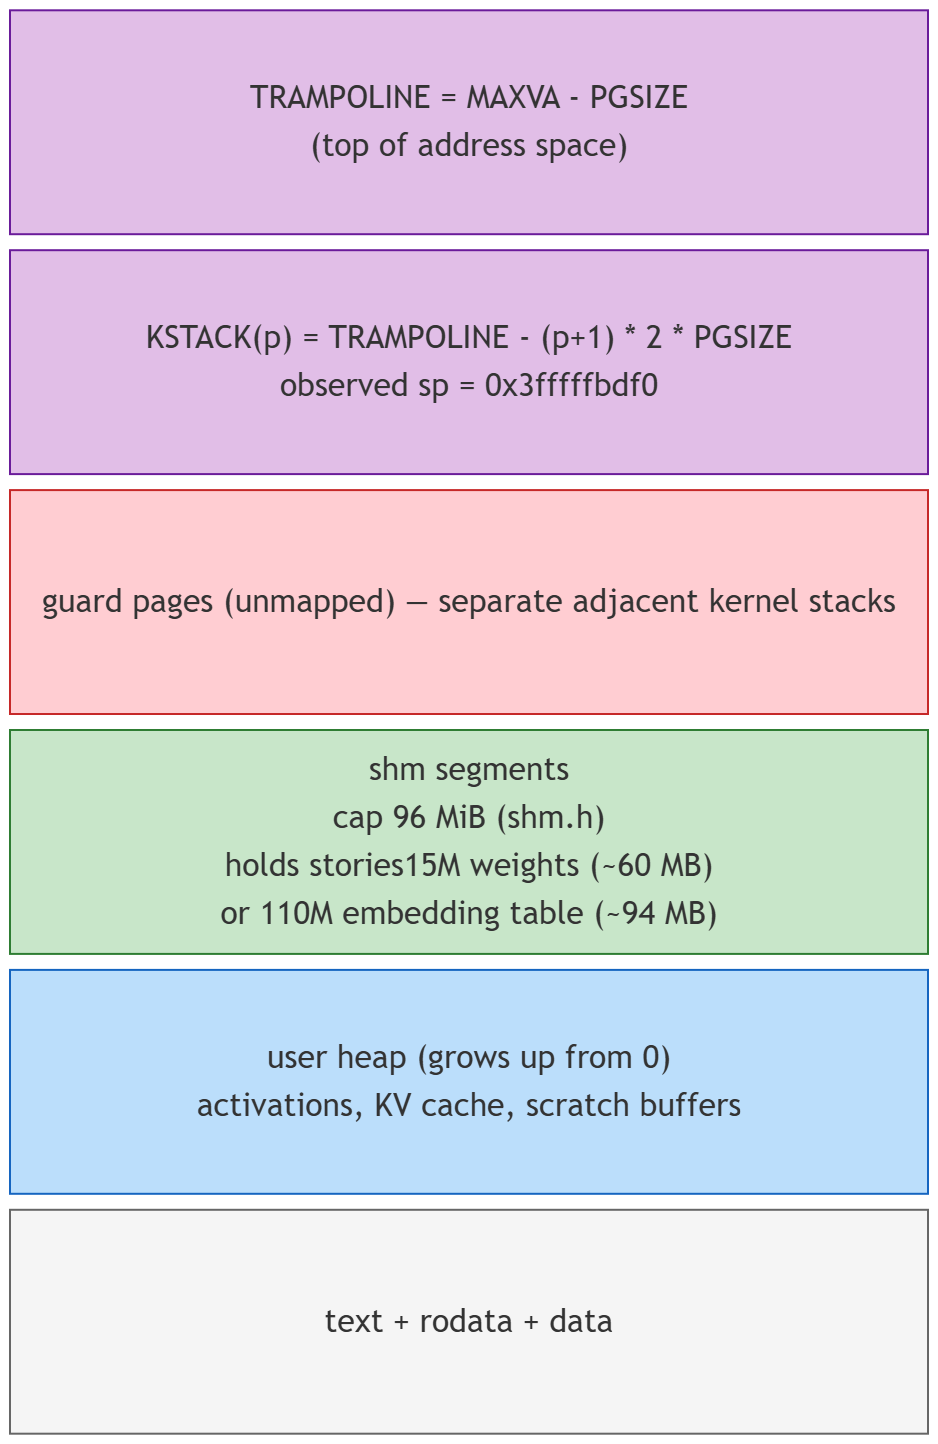
\includegraphics[width=0.75\textwidth]{figures/F6.png}

\caption{Node memory map. \texttt{MAXVA = 256\,GB ($2^{38}$)}. \texttt{stories15M} fits in 256\,MB RAM; \texttt{stories110M} does not, and is shaded in the ring. The 96\,MiB segment cap in \texttt{shm.h} is chosen so the 110M embedding table ($\sim$94\,MB) fits in one segment.}
\label{fig:F6}
\end{figure}

\begin{lstlisting}[language=Mermaid,caption={F6 Mermaid source.}]
block-beta
    columns 3
    block:Trampoline:1
        TR["TRAMPOLINE = MAXVA - PGSIZE"]
    end
    block:KStack:2
        KS["KSTACK(p) = TRAMPOLINE - (p+1)*2*PGSIZE<br/>observed sp = 0x3fffffbdf0"]
    end
    block:Guard:2
        G["unmapped guard pages"]
    end
    block:SharedMem:3
        SHM["shm segments<br/>cap 96 MiB (shm.h)<br/>holds stories15M weights (~60 MiB)<br/>or 110M embedding (~94 MiB)"]
    end
    block:UserHeap:3
        UH["user heap (grows up from 0)<br/>activations, KV cache, scratch"]
    end
    block:Text:3
        TX["text + rodata + data"]
    end
\end{lstlisting}

\subsection{F7: Baseline Graphs}

Figures~\ref{fig:F7_throughput}--\ref{fig:F7_ring_gen} plot the baseline measurements from Section~\ref{sec:baseline}: single-node throughput, E2EL, inference time, TTFT (F7a--F7d), and ring throughput and generation time at 2 and 3 workers (F7e, F7f).

\begin{figure}[H]
\centering
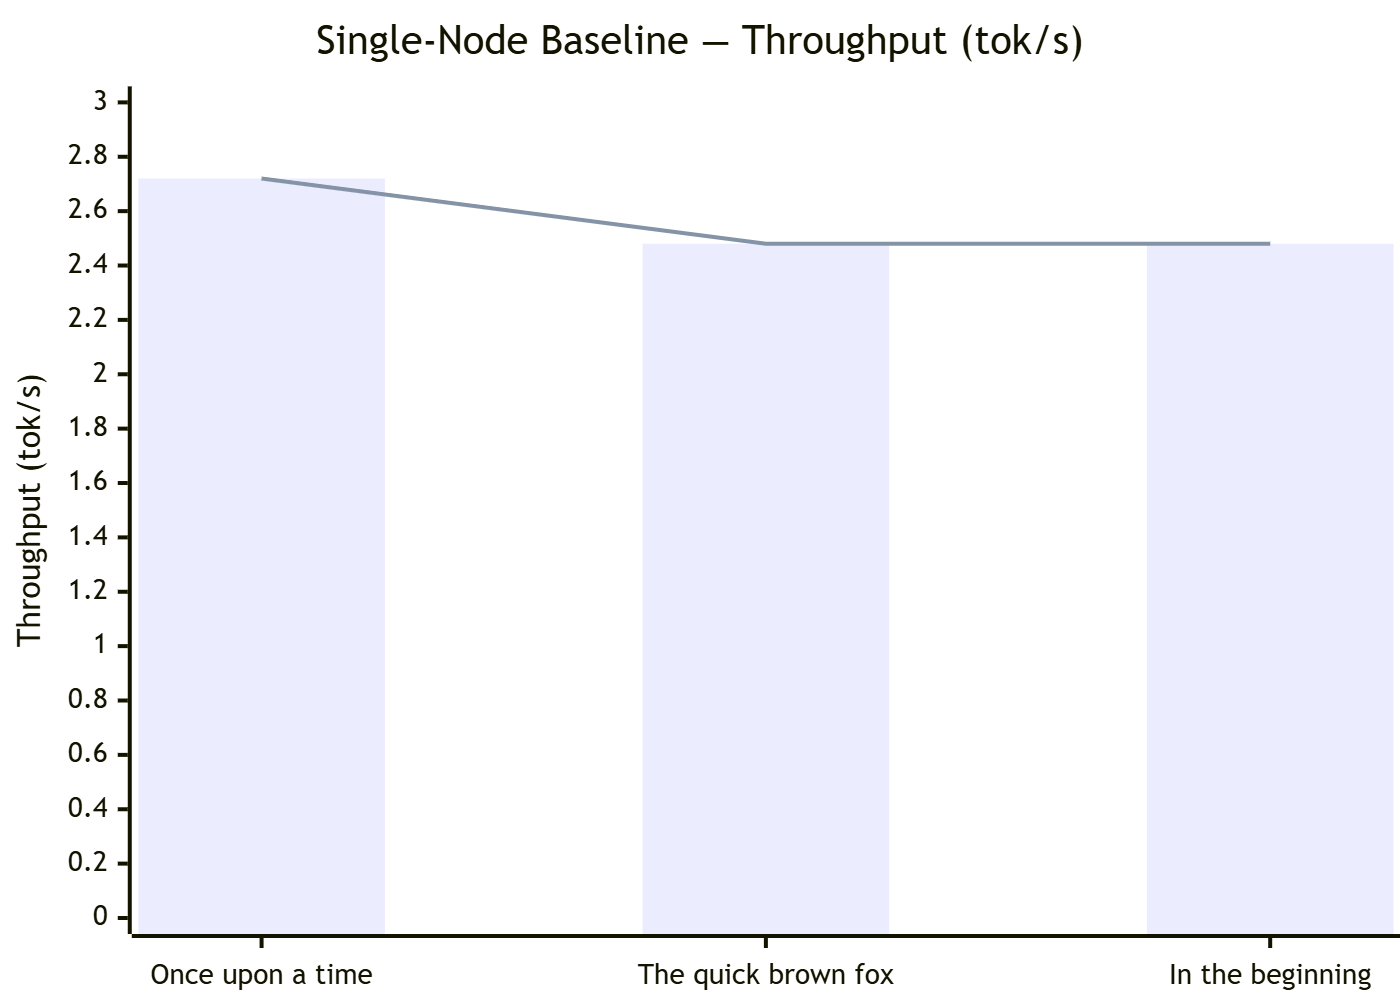
\includegraphics[width=0.75\textwidth]{figures/F7a.png}

\caption{Single-node baseline: throughput (tok/s).}
\label{fig:F7_throughput}
\end{figure}

\begin{figure}[H]
\centering
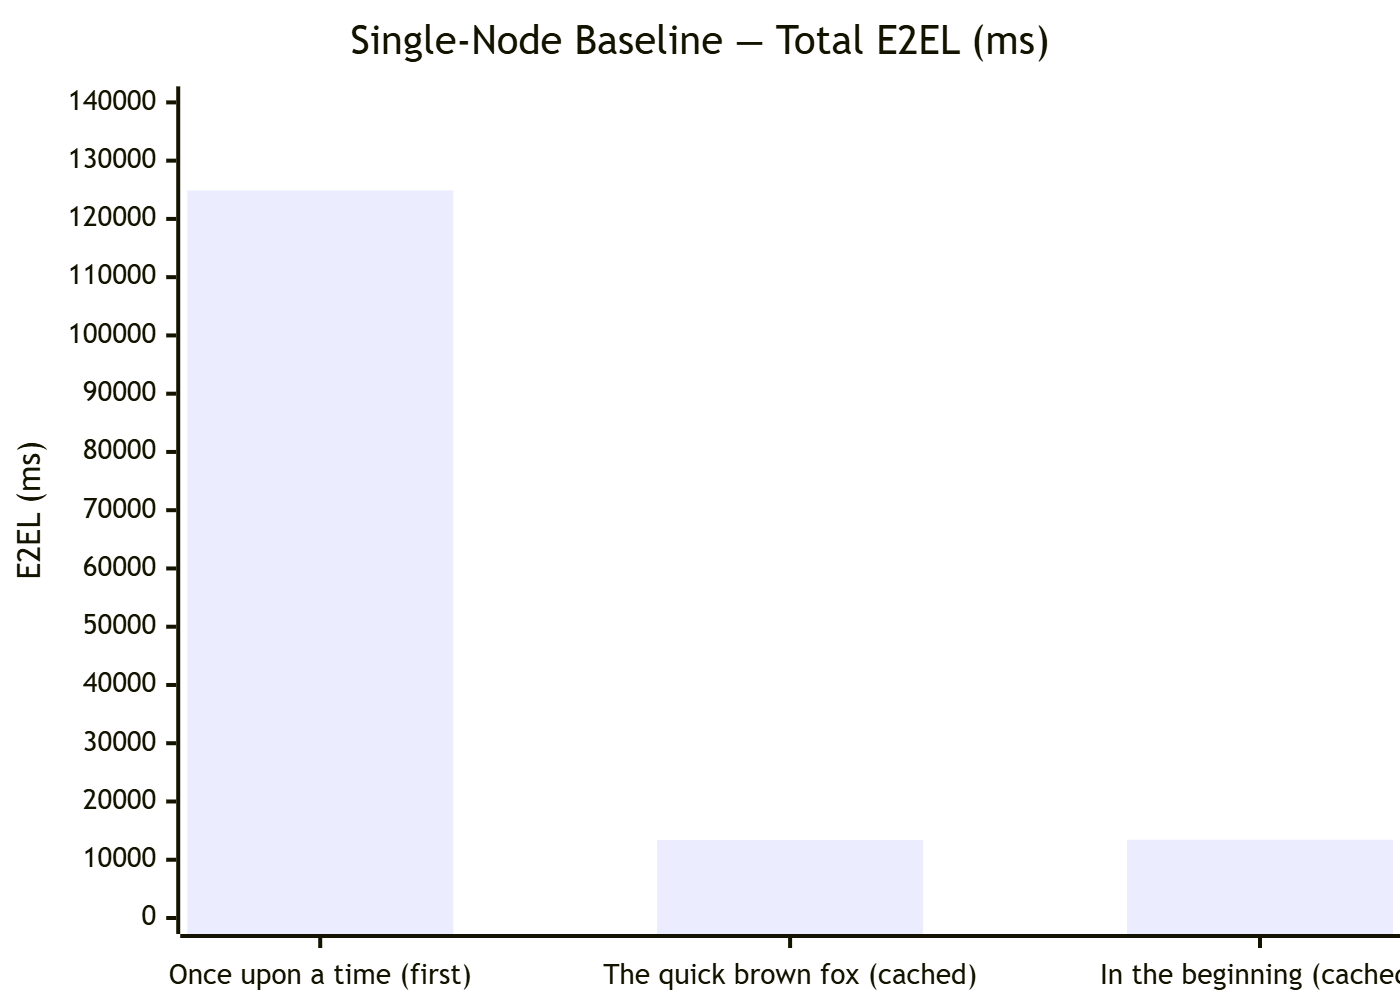
\includegraphics[width=0.75\textwidth]{figures/F7b.png}

\caption{Single-node baseline: total E2EL (ms).}
\label{fig:F7_e2el}
\end{figure}

\begin{figure}[H]
\centering
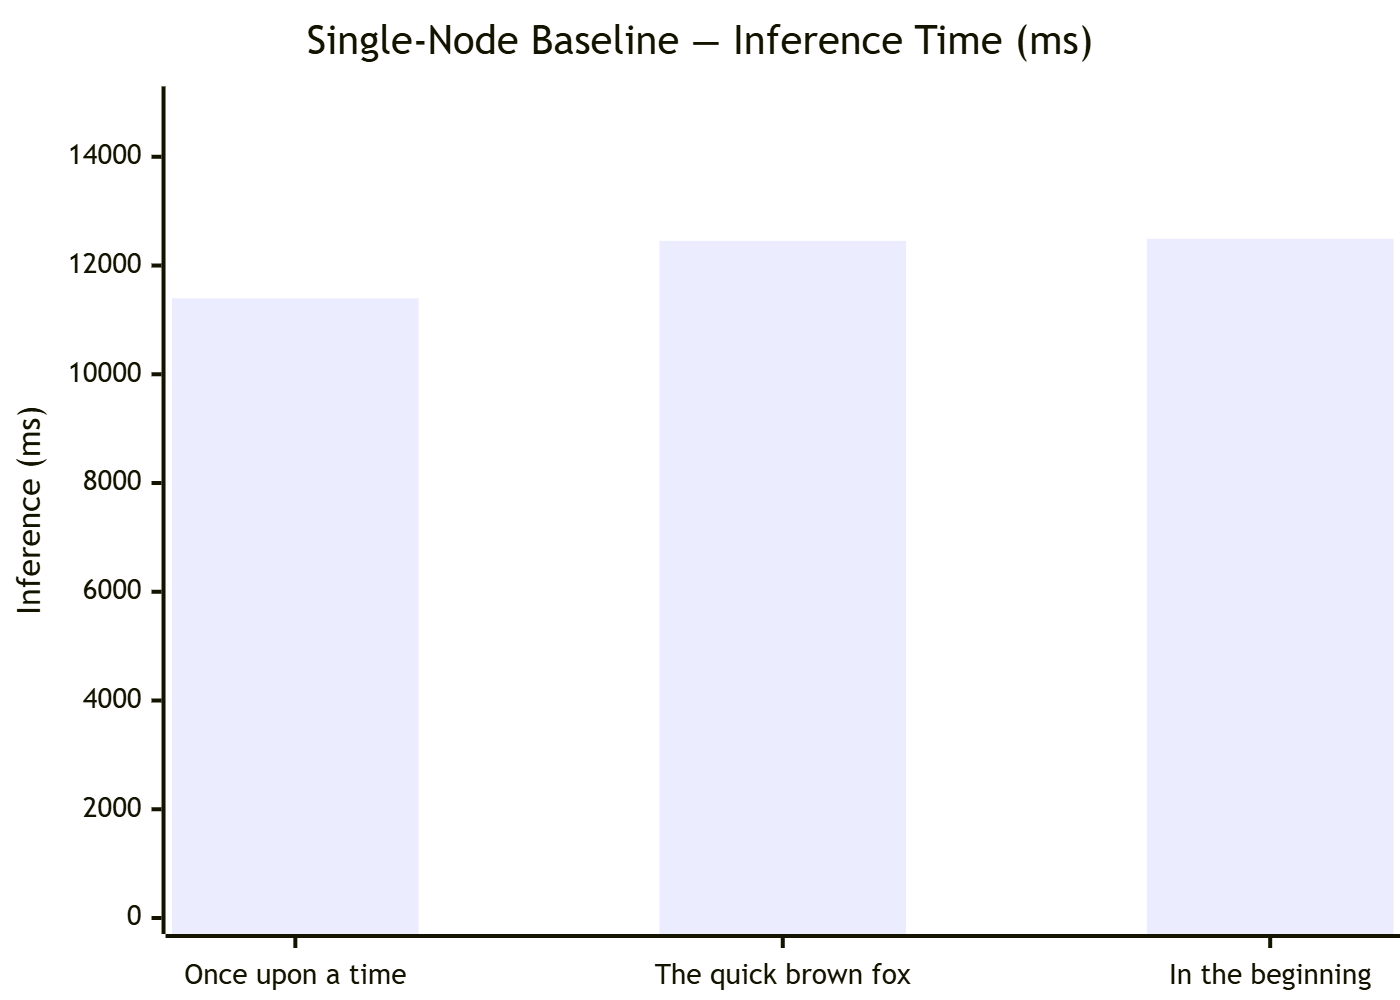
\includegraphics[width=0.75\textwidth]{figures/F7c.png}

\caption{Single-node baseline: inference time (ms).}
\label{fig:F7_inf}
\end{figure}

\begin{figure}[H]
\centering
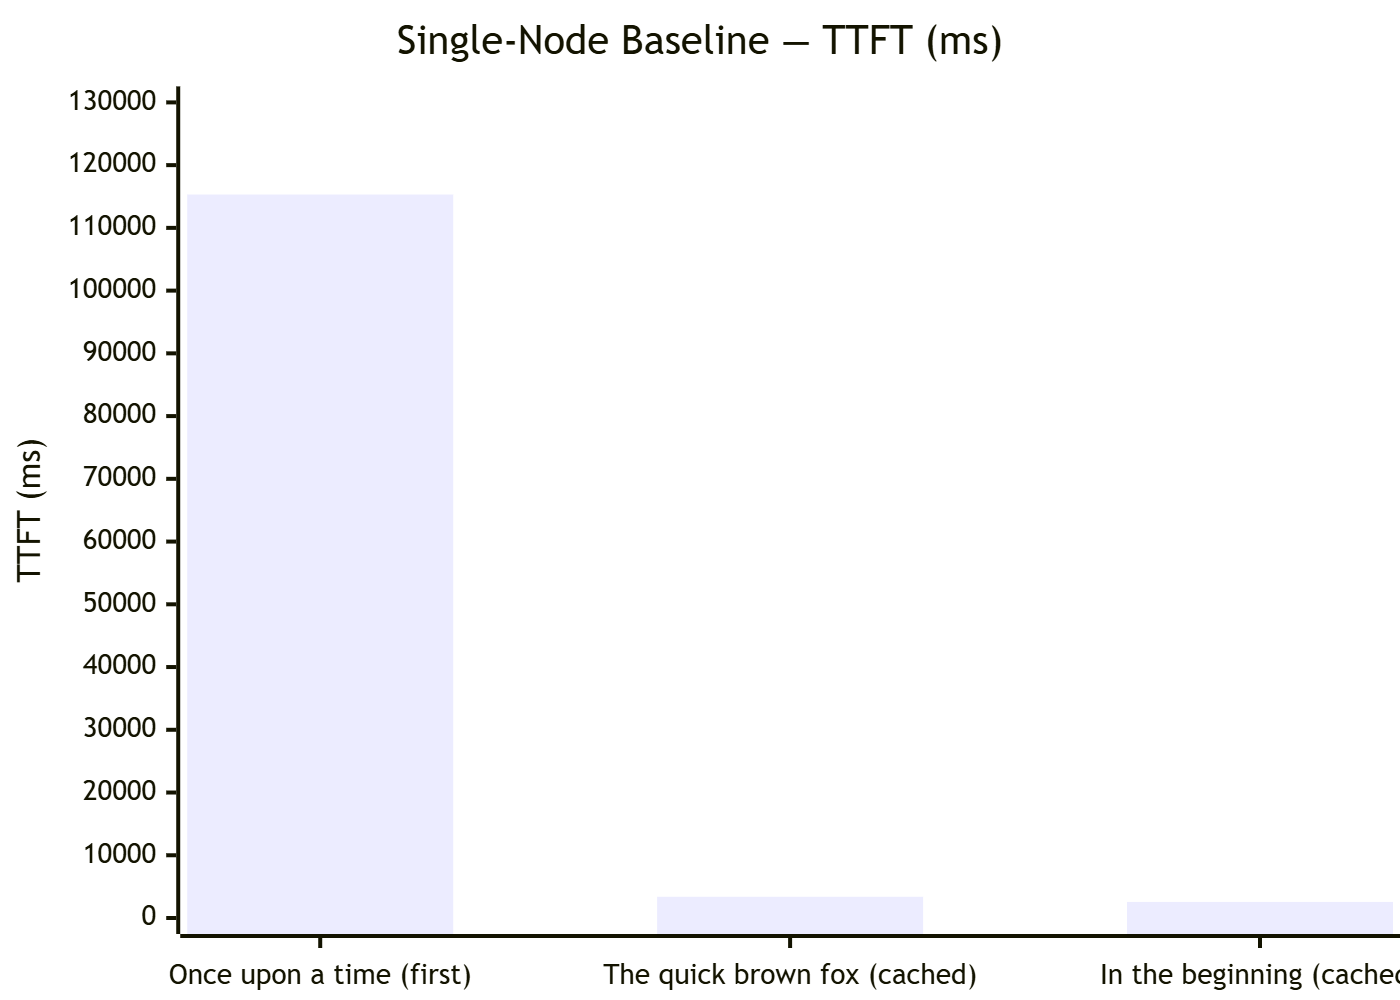
\includegraphics[width=0.75\textwidth]{figures/F7d.png}

\caption{Single-node baseline: TTFT (ms).}
\label{fig:F7_ttft}
\end{figure}

\begin{figure}[H]
\centering
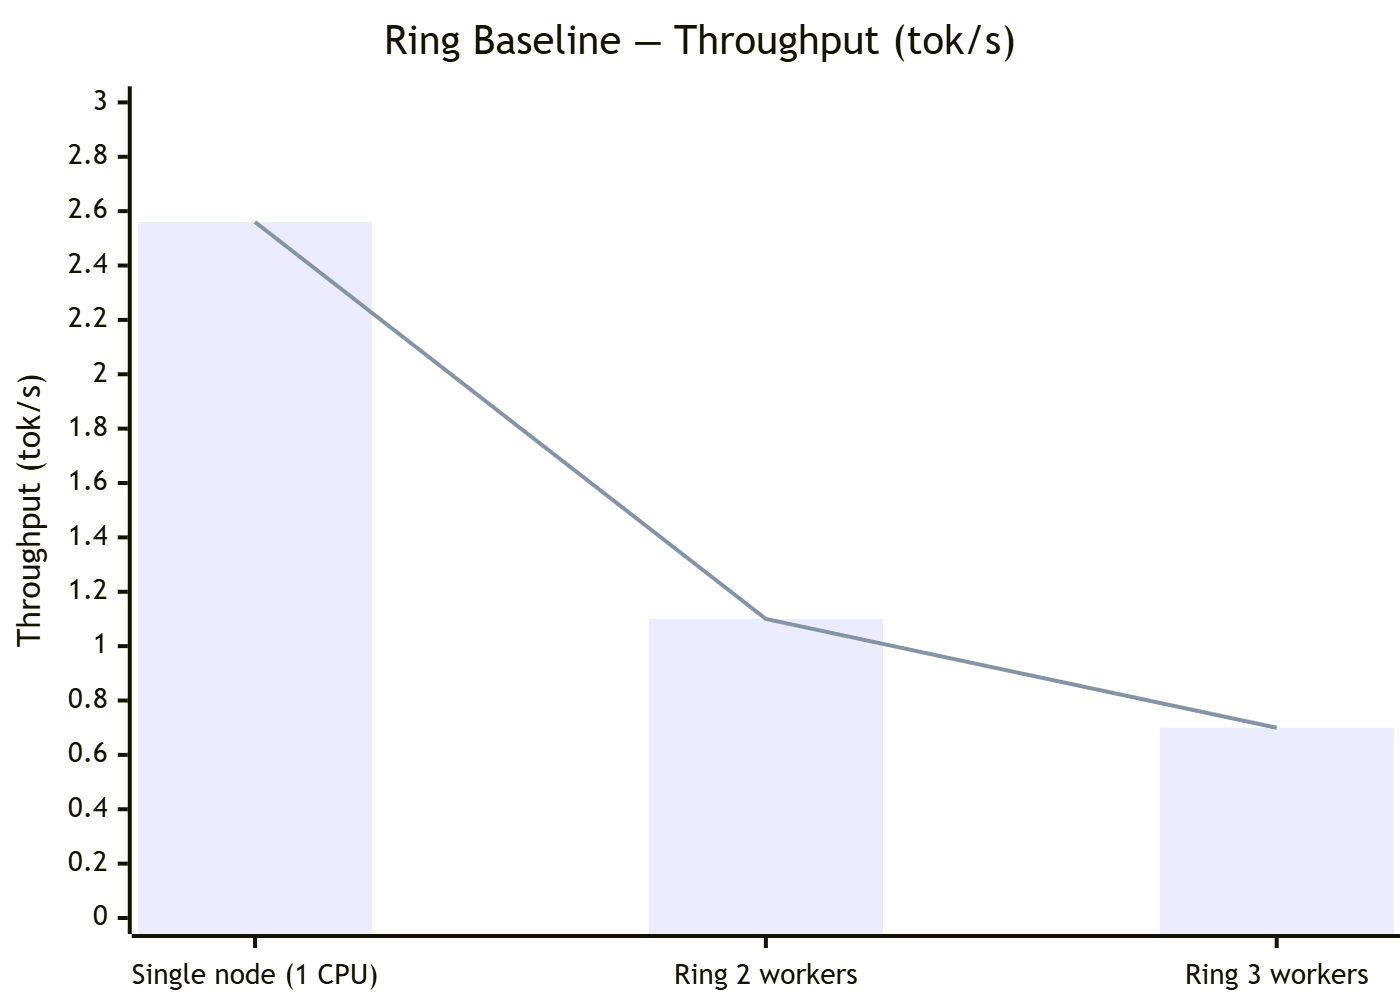
\includegraphics[width=0.75\textwidth]{figures/F7e.png}

\caption{Ring baseline: throughput (tok/s) for single node (1 CPU), ring 2 workers, and ring 3 workers.}
\label{fig:F7_ring_thr}
\end{figure}

\begin{figure}[H]
\centering
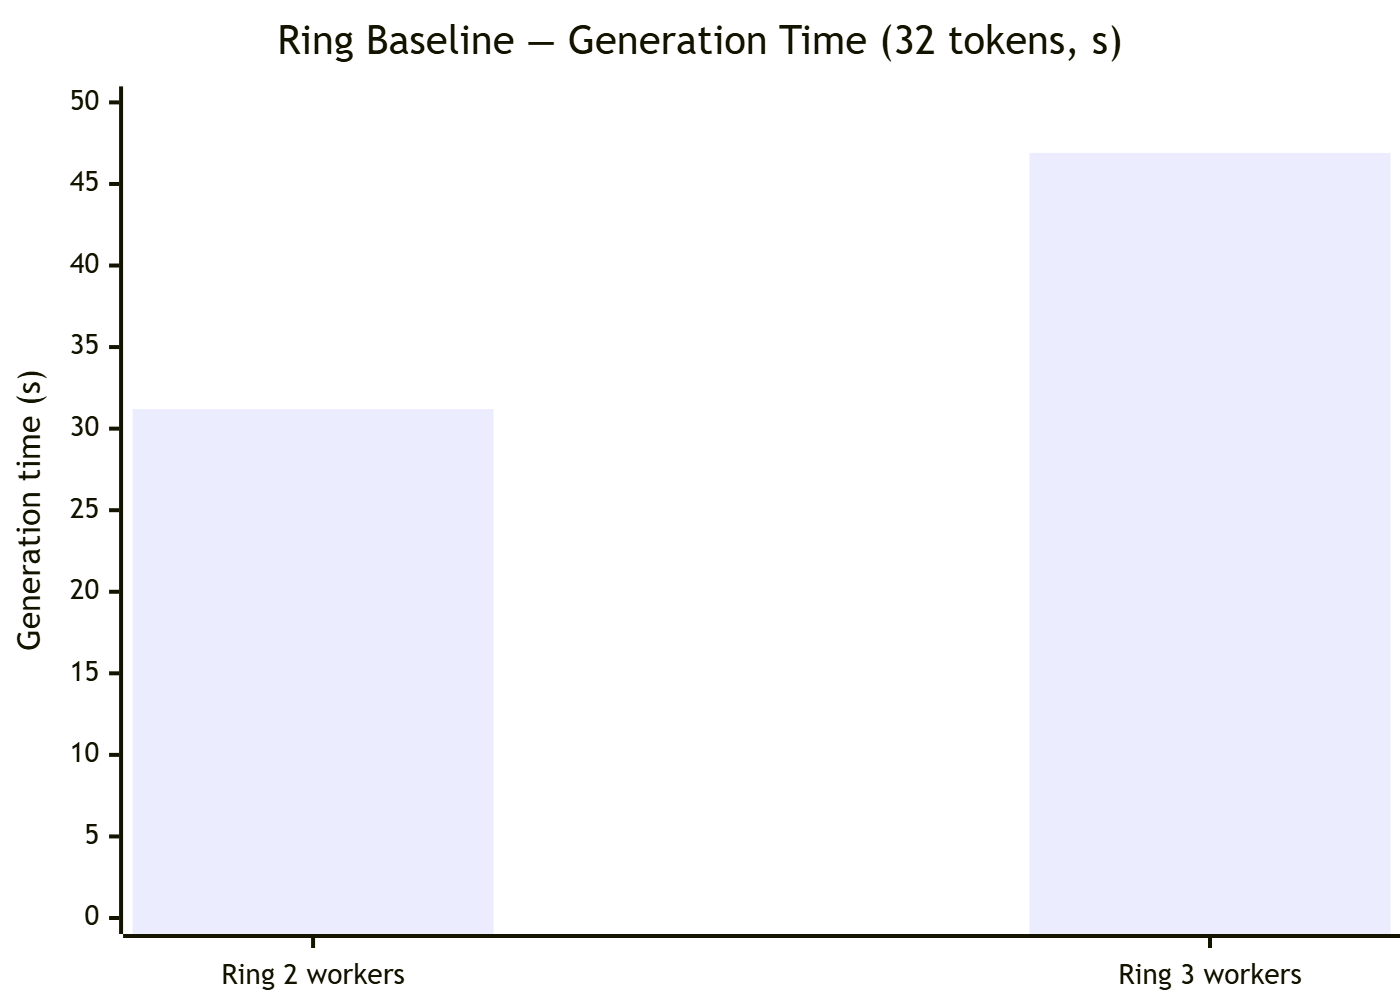
\includegraphics[width=0.75\textwidth]{figures/F7f.png}

\caption{Ring baseline: generation time (32 tokens, s) for ring 2 and 3 workers.}
\label{fig:F7_ring_gen}
\end{figure}

\begin{lstlisting}[language=Mermaid,caption={F7 Mermaid source (representative throughput chart).}]
xychart-beta
    title "Ring Baseline — Throughput (tok/s)"
    x-axis ["Single node (1 CPU)", "Ring 2 workers", "Ring 3 workers"]
    y-axis "Throughput (tok/s)" 0 --> 3
    bar [2.56, 1.1, 0.7]
    line [2.56, 1.1, 0.7]
\end{lstlisting}

% ============================================================
\section{Difference From Upstream}
% ============================================================

The system ships 59 syscalls. Stock xv6 has 21, so 38 were added on top of stock. The original repo \texttt{xv6-llm-runtime-arch} already has 47 syscalls (including the three hardware-counter syscalls \texttt{rdcycle}, \texttt{rdtime}, \texttt{rdinstret}), so only 12 are new relative to that ancestor: \texttt{setrlimit}, \texttt{getrlimit}, \texttt{capget}, \texttt{capdrop}, \texttt{getentropy}, \texttt{getuid}, \texttt{geteuid}, \texttt{setuid}, \texttt{seteuid}, \texttt{recvtimeo}, \texttt{ip}, \texttt{udp\_bulk}.

\subsection{Added Syscall Table}

\begin{longtable}{@{}p{0.7cm}p{3.2cm}p{9.5cm}@{}}
\toprule
\textbf{\#} & \textbf{Name} & \textbf{Description} \\
\midrule
\endfirsthead
\toprule
\textbf{\#} & \textbf{Name} & \textbf{Description} \\
\midrule
\endhead
22 & \texttt{trace} & Trace syscall (MIT 6.828 lab) \\
23 & \texttt{interpose} & Syscall interposition (lab) \\
24 & \texttt{sigalarm} & Signal alarm (lab) \\
25 & \texttt{sigreturn} & Signal return (lab) \\
26 & \texttt{symlink} & Symbolic link (lab) \\
27 & \texttt{mmap} & Memory map (lab) \\
28 & \texttt{munmap} & Memory unmap (lab) \\
29 & \texttt{bind} & Bind UDP port \\
30 & \texttt{unbind} & Unbind UDP port \\
31 & \texttt{send} & Send UDP datagram \\
32 & \texttt{recv} & Receive UDP datagram \\
33 & \texttt{pgpte} & Page table entry inspection (lab) \\
34 & \texttt{kpgtbl} & Kernel page table inspection (lab) \\
35 & \texttt{shmget} & Shared memory get \\
36 & \texttt{shmat} & Shared memory attach \\
37 & \texttt{shmdt} & Shared memory detach \\
38 & \texttt{shmctl} & Shared memory control \\
39 & \texttt{rdcycle} & Read cycle counter \\
40 & \texttt{rdtime} & Read time \\
41 & \texttt{rdinstret} & Read instructions retired \\
42 & \texttt{getramused} & Get RAM used \\
43 & \texttt{setrlimit} & Set resource limit (POSIX.1-2017) \\
44 & \texttt{getrlimit} & Get resource limit (POSIX.1-2017) \\
45 & \texttt{capget} & Get capabilities (POSIX.1e) \\
46 & \texttt{capdrop} & Drop capability (POSIX.1e) \\
47 & \texttt{getentropy} & Get entropy bytes (POSIX.1-2024) \\
48 & \texttt{getuid} & Get user ID (POSIX.1-2017) \\
49 & \texttt{geteuid} & Get effective user ID (POSIX.1-2017) \\
50 & \texttt{setuid} & Set user ID (POSIX.1-2017) \\
51 & \texttt{seteuid} & Set effective user ID (POSIX.1-2017) \\
52 & \texttt{recvtimeo} & Receive with timeout \\
53 & \texttt{ip} & Get node IP \\
54 & \texttt{thread\_create} & Create thread \\
55 & \texttt{thread\_join} & Join thread \\
56 & \texttt{thread\_exit} & Exit thread \\
57 & \texttt{yield} & Yield CPU \\
58 & \texttt{setpriority} & Set process priority \\
59 & \texttt{udp\_bulk} & Declare bulk UDP flow (CAP\_NET\_ADMIN) \\
\bottomrule
\caption{The 38 syscalls added on top of stock xv6.}
\end{longtable}

\subsection{File Classification}

Each file is placed in \emph{exactly one} of the rubric's five categories.

\paragraph{Networking.}
\texttt{kernel/net.h}, \texttt{kernel/e1000\_dev.h}, \texttt{user/netecho.c}, \texttt{user/nettest.c}, \texttt{user/ftp-client.c/.h}, \texttt{user/testftp.c}, \texttt{user/rpc.c/.h}, \texttt{user/xdr.c/.h}.

\paragraph{Distributed Inference.}
\texttt{user/discovery.c/.h}, \texttt{user/distinf.c/.h}, \texttt{user/shard.c/.h}, \texttt{user/llama.c}, \texttt{kernel/shm.h}, \texttt{user/testshm.c}, \texttt{user/threadtest.c}, \texttt{user/mutex.c}.

\paragraph{Model Computation.}
\texttt{user/llama\_core.c/.h}, \texttt{user/xmath.c/.h}, \texttt{user/xmath\_test\_cases.h}, \texttt{user/testxmath.c}, \texttt{user/xstdlib.c/.h}, \texttt{user/testxstdlib.c}, \texttt{user/xstrlib.c/.h}.

\paragraph{Hardening.}
\texttt{kernel/stackguard.c}, \texttt{kernel/random.c/.h}, \texttt{kernel/rlimit.h}, \texttt{kernel/capability.h}, \texttt{user/canarytest.c}, \texttt{user/wxtest.c}, \texttt{user/wxbad.c}, \texttt{user/stackguard.c}, \texttt{user/idtest.c}, \texttt{user/rlimittest.c}, \texttt{user/randtest.c}, \texttt{user/aslrtest.c}, \texttt{user/sha256.c/.h}, \texttt{user/threadstack.c}.

\paragraph{Measurement.}
\texttt{user/perf.c/.h}, \texttt{user/testperf.c}.

\noindent\textbf{Note:} \texttt{kernel/shm.h}, \texttt{user/testshm.c}, \texttt{user/threadtest.c}, and \texttt{user/mutex.c} are placed in Distributed Inference, not Hardening, because they support the inference runtime (shared-memory weight cache, inference threads), not the security surface.

% ============================================================
\section{Baseline Measurements}
\label{sec:baseline}
% ============================================================

\subsection{Method}

All measurements were taken at temperature $0$ (\texttt{-t 0}), 32 steps, model \texttt{stories15M.bin} (id 1), and CPU count 1 (\texttt{XV6\_CPUS=1 ./boot.sh}). QEMU does not model real hardware timing, so guest cycle counts are not real-world timings; all figures below are reported as \emph{ratios and relative differences}, not absolute microseconds.

\textbf{Primary metric caveat.} The handout specifies instructions retired as the primary metric, wrapped by \texttt{user/perf.c}. In the shipped tree, no user-space program actually calls \texttt{rdcycle} or \texttt{rdinstret}: the syscalls exist in \texttt{kernel/syscall.h} and are exposed in \texttt{user/user.h}, but the profiling library \texttt{user/perf.c} uses only \texttt{rdtime()} (wall-clock milliseconds, 10\,MHz timebase). We attempted to capture instructions retired via the shipped benchmark, but \texttt{testperf} runs a nested-function-call microbenchmark, not the LLM workload, and no shipped program prints the counters for LLM inference. \textbf{Throughput (tok/s) and wall-clock time (ms) are therefore reported as the primary available metrics}, with the caveat that this differs from the handout's intended primary metric. This discrepancy is itself an Observation (see Section~\ref{sec:obs}).

\textbf{CPU-count caveat.} The ring nodes ran with the simulator's default of 8 virtual CPUs each (via \texttt{--smp 2} in our runs the simulator reduced this), while the single node ran with 1. Ring-vs-single ratios ($2.3\times$ and $3.7\times$) are therefore indicative, not a CPU-controlled comparison. Each table row notes the core count at which it was taken.

\subsection{Instructions Retired --- Not Captured}

As noted above, \texttt{rdinstret} and \texttt{rdcycle} are implemented as syscalls in \texttt{kernel/syscall.h} (numbers 41 and 39) and declared for user-space use in \texttt{user/user.h}, but no shipped user program invokes them for the LLM workload. We attempted \texttt{perf llama -t 0 -n 32 -i "Once upon a time"} but the command returned \texttt{exec perf failed} (no such binary). The \texttt{testperf} binary runs a nested-function-call benchmark, not the LLM. Instructions retired and cycles were therefore \textbf{not captured} in this milestone.

\subsection{Single Node (\texttt{XV6\_CPUS=1})}

All rows were taken at \texttt{XV6\_CPUS=1}. The first row is a fresh boot (cold cache: the 60\,MB checkpoint is fetched over emulated UDP); the second and third rows are subsequent \texttt{llama} invocations in the \emph{same} boot, where the weights are already in shared memory and the fetch is skipped.

\begin{table}[H]
\centering
\begin{tabular}{lrrrr}
\toprule
\textbf{Prompt} & \textbf{Throughput (tok/s)} & \textbf{E2EL (ms)} & \textbf{Inference (ms)} & \textbf{TTFT (ms)} \\
\midrule
Once upon a time (first, cold) & 2.72 & 124,887 & 11,396 & 115,319 \\
The quick brown fox (cached)  & 2.48 & 13,378  & 12,453 & 3,377 \\
In the beginning (cached)     & 2.48 & 13,446  & 12,493 & 2,556 \\
\midrule
\textbf{Mean}                 & \textbf{2.56} & --- & --- & --- \\
\bottomrule
\end{tabular}
\caption{Single-node baseline. First row cold; rows 2--3 warm (weights cached in shared memory).}
\end{table}

\subsection{Ring}

\begin{table}[H]
\centering
\begin{tabular}{lrr}
\toprule
\textbf{Metric} & \textbf{Ring 2 workers} & \textbf{Ring 3 workers} \\
\midrule
Throughput (tok/s)          & 1.1 & 0.7 \\
Generation (32 tokens, s)   & 31.2 & 46.9 \\
Ring RTT ($\mu$s)           & 870,302 & 1,410,649 \\
compute ($\mu$s)            & 134,204 & 189,875 \\
network ($\mu$s)            & 736,098 & 1,220,774 \\
Master ($\mu$s)             & 89,034  & 116,128 \\
\midrule
Ring vs Single (mean 2.56 tok/s) & $2.3\times$ & $3.7\times$ \\
\bottomrule
\end{tabular}
\caption{Ring baseline at 2 and 3 workers on the first prompt (``Once upon a time'').}
\end{table}

\textbf{Relative finding.} Throughput \emph{dropped} from 2 to 3 workers ($1.1 \to 0.7$ tok/s) despite each worker holding fewer layers (3 each $\to$ 2 each). Network/RPC hop overhead increased from 736,098 to 1,220,774\,$\mu$s (a 66\% increase), which outweighs the per-worker compute savings. This pipeline configuration does not scale favourably past 2 workers on this workload and hardware.

% ============================================================
\section{Observations Log}
\label{sec:obs}
% ============================================================

The following observations were made while reading the source and disassembly. Each is cited to a specific file and line (or symbol). No fixes are made in this milestone.

\begin{enumerate}[leftmargin=*]

\item \textbf{\texttt{kernel/syscall.h} (comment preceding \texttt{SYS\_thread\_create}, line 54).}
The comment block documents a real historical bug: the thread/scheduler syscalls (\texttt{thread\_create}, \texttt{thread\_join}, \texttt{thread\_exit}, \texttt{yield}) were originally numbered 43--47 on a separate branch. On the branch that later added the POSIX resource-limit block (\texttt{setrlimit}, \texttt{getrlimit}, \texttt{capget}, \texttt{capdrop}, \texttt{getentropy}), the same numbers 43--47 were reused. Because \texttt{syscalls[]} uses designated initializers, the collision was not a compile error --- ``the later initializer silently wins'' --- so five POSIX syscalls were silently dispatching to the wrong (thread/scheduler) handlers. \textbf{Severity: high.} This is a real defect, not a documentation issue.

\item \textbf{\texttt{user/discovery.h:116}.}
The field \texttt{last\_seen.ms} is named for milliseconds but is actually given \emph{ticks}. The unit suffix is misleading.

\item \textbf{\texttt{user/rpc.h:46}.}
The doc-comment above \texttt{PROC\_SET\_NEIGHBOR} is a copy-paste of the \texttt{\_CAP\_ADVERTISE} comment --- the procedure description does not match the procedure it documents.

\item \textbf{\texttt{user/distinf.h:57}.}
The comment says the header is ``13 words'' but the macro \texttt{ASSIGN\_LAYERS\_WORDS} is 14.

\item \textbf{\texttt{user/distinf.h:35}.}
The comment says little-endian, but the code uses XDR big-endian for the same payload.

\item \textbf{\texttt{user/discovery.h:33}.}
\texttt{MASTER\_POLL\_MS} is a dead constant --- defined but never referenced.

\item \textbf{\texttt{user/discovery.c:400}.}
The comment says ``block forever'' but the code uses a 5000\,ms timeout.

\item \textbf{\texttt{user/discovery.c:794}.}
A capability-claim timeout TODO that has not been resolved.

\item \textbf{\texttt{kernel/net.h} (top of file).}
The file's own top comment admits a real historical bug: without the \texttt{\#ifndef XV6\_IP\_D} / \texttt{XV6\_MAC\_LAST} defaults it defines, \texttt{kernel/e1000.c} and \texttt{kernel/net.c} failed to compile outside the multi-node build targets, ``which is what silently made the L1 kernel gate unbuildable on this branch.''

\item \textbf{\texttt{user/distinf.h} (top-of-file comment).}
The comment block documents an RFC~4506 encoding inconsistency between new payloads (which follow XDR) and three legacy discovery payloads (\texttt{worker\_info\_t}, \texttt{set\_neighbor\_t}, \texttt{cap\_ack\_t}) that are raw little-endian structs. The comment says this divergence is ``recorded in README.md and left alone'' rather than churning working, gated code.

\item \textbf{\texttt{user/perf.c}, \texttt{user/llama.c}, \texttt{user/schedtest.c}.}
The syscalls \texttt{rdcycle} (39) and \texttt{rdinstret} (41) are implemented in the kernel and declared for user-space use in \texttt{user/user.h}, but \emph{no} shipped user-space program actually invokes them. Every profiling number printed by \texttt{llama} --- \texttt{Total Time}, \texttt{Inference}, \texttt{TTFT}, tok/s --- comes from \texttt{rdtime()} only (wall-clock milliseconds). The handout describes \texttt{rdcycle}/\texttt{rdinstret} as ``wrapped by \texttt{user/perf.c}'', but the wrapper is not present in this tree. This discrepancy is the reason instructions retired could not be reported as the primary metric (see Section~\ref{sec:baseline}).

\end{enumerate}

% ============================================================
\section{Related Systems}
% ============================================================

\begin{table}[H]
\centering
\small
\begin{tabular}{lcccccc}
\toprule
\textbf{Feature} & \textbf{Stock xv6} & \textbf{Linux} & \textbf{Petals} & \textbf{Exo} & \textbf{llama.cpp RPC} & \textbf{Orig repo} \\
\midrule
Syscalls              & 21     & $\sim$450 & N/A   & N/A   & N/A   & 47 \\
Network stack         & No     & Full      & Yes   & Yes   & Yes   & Yes \\
Threads               & No     & Yes       & Yes   & Yes   & Yes   & Yes \\
Shared memory         & No     & Yes       & N/A   & N/A   & N/A   & Yes \\
Resource limits       & No     & Yes       & N/A   & N/A   & N/A   & No \\
Capabilities          & No     & Yes       & N/A   & N/A   & N/A   & Yes \\
Entropy source        & No     & Yes       & N/A   & N/A   & N/A   & No \\
W\^{}X                & No     & Yes       & N/A   & N/A   & N/A   & Yes \\
Multi-node ring       & No     & N/A       & Yes   & Yes   & Yes   & No \\
Weight fetch over net & No     & N/A       & Yes   & Yes   & Yes   & Yes \\
Discovery + registration & No  & N/A       & Yes   & Yes   & Yes   & No \\
RPC / XDR             & No     & N/A       & Yes   & Yes   & Yes   & No \\
Hardware counters     & No     & Yes       & N/A   & N/A   & N/A   & Yes (\texttt{rdcycle}/\texttt{rdtime}/\texttt{rdinstret}) \\
Real hardware support & Yes    & Yes       & Yes   & Yes   & Yes   & Unverified \\
GPU support           & No     & Yes       & Yes   & Yes   & Yes   & No \\
Auditable in one sitting & Yes & No        & No    & No    & No    & Yes \\
\bottomrule
\end{tabular}
\caption{Related systems compared in both directions.}
\end{table}

\noindent\textbf{Notes.}
\begin{itemize}[leftmargin=*]
\item GPipe and PipeDream are training systems, not inference systems, and are not used as comparison points.
\item Petals runs on volunteer GPUs over the public Internet, BitTorrent-style, not on a dedicated cluster.
\item Per the Exo README, peer discovery in Exo is not authenticated; this system's PSK/HMAC registration is a feature Exo does not have.
\item The ``Orig repo'' column refers to \url{https://github.com/syedtaha22/xv6-llm-runtime-arch}.
\end{itemize}

\noindent\textbf{What each external system does that this system does not, and vice versa.}
\begin{itemize}[leftmargin=*]
\item \textbf{Stock xv6}: provides nothing beyond a minimal teaching UNIX --- no networking stack, no capability/rlimit model, no RPC layer. This system adds the entire network stack (row~1), the hardening set (row~8), and the RPC/XDR/discovery/sharding/inference stack (rows 2--7).
\item \textbf{Linux}: provides full POSIX.1e capability sets, real uid/gid permissions, mature TCP/IP with congestion control, production-grade scheduling, and ASLR. This system does none of those; the value of the xv6 base is auditability --- every layer is visible and every defense attributable.
\item \textbf{Petals}: runs across untrusted volunteer GPUs with DHT-based discovery, dynamic join/leave, and Byzantine-fault tolerance. This system runs pipeline-parallel inference on a from-scratch OS kernel it also hardens itself; Petals assumes a trusted host OS.
\item \textbf{Exo}: focuses on the ML-serving layer over trusted hosts. This system implements the full stack including OS-level security and RPC transport that Exo assumes exist.
\item \textbf{llama.cpp RPC}: provides production GPU-backed RPC inference across trusted machines. This system demonstrates the RPC transport, wire serialization, discovery/heartbeat, and kernel hardening on bare-metal-equivalent hardware, none of which llama.cpp RPC touches.
\end{itemize}

% ============================================================
\section{Contributions}
% ============================================================

Beyond the eight required tasks, the team believes the following are worth merging into the main project.

\begin{enumerate}[leftmargin=*]
\item \textbf{Raise the ring simulator's \texttt{--shard-timeout} default from 900\,s to 1800\,s.}
\textbf{Evidence:} on the team's hardware (i5-8350U, 4 cores / 8 threads), the 35\,MB embedding fetch per worker repeatedly exceeded 900\,s under three-guest contention, causing \texttt{FAIL -- never assigned layers within 900s}. With \texttt{--shard-timeout 1800} the same run consistently \texttt{PASS}es. A safer default removes a non-obvious failure mode for anyone running the simulator on consumer hardware.

\item \textbf{Document the \texttt{.venv} activation requirement for \texttt{distinf\_sim.py} in \texttt{README.md} and the runbook.}
\textbf{Evidence:} \texttt{server/distinf\_sim.py} launches \texttt{mcast\_switch.py} using \texttt{sys.executable} (the interpreter that ran the simulator). If the caller forgot to activate \texttt{.venv}, \texttt{mcast\_switch.py} crashes silently on \texttt{ModuleNotFoundError: coloredlogs}, which surfaces downstream only as \texttt{arp\_lookup: resolution timed out for 0xa000001}. This cost the team hours to diagnose and is trivially preventable by a README note.

\item \textbf{Fix the syscall-numbering collision documented in \texttt{kernel/syscall.h} (Observation~1).}
\textbf{Evidence:} the comment block itself records that syscalls 43--47 silently overrode the POSIX resource-limit handlers with thread/scheduler handlers. This is a real defect, not a documentation issue. Renumbering the thread block to 54--57 (as the code already does on this branch) and adding a compile-time duplicate check would prevent recurrence.

\item \textbf{Add an inline unit test for \texttt{ASSIGN\_LAYERS\_WORDS} vs.\ the doc-comment (Observation~4).}
\textbf{Evidence:} the comment says 13 words, the macro is 14. A two-line \texttt{\_Static\_assert} would catch the next drift.

\item \textbf{Add the F3 worker-lifecycle state diagram to \texttt{diagrams/} and remove or correct \texttt{state\_diagram.png}.}
\textbf{Evidence:} the existing hand-drawn diagram disagrees with the code on three points (Section~6.3). The Mermaid source in this report is drawn directly from \texttt{discovery.h} states and \texttt{discovery.c} transitions, and is version-controllable.
\end{enumerate}

% ============================================================
\appendix
\section{Appendices}
% ============================================================

\subsection{Bring-Up Transcripts}

The three required transcripts (Section~3.1 of the handout) are reproduced below as screenshots. The full plain-text transcripts are committed to the repository as \texttt{single\_node\_transcript.txt}, \texttt{ring\_transcript.txt}, and \texttt{weightfetch\_transcript.txt}.

\begin{figure}[H]
\centering
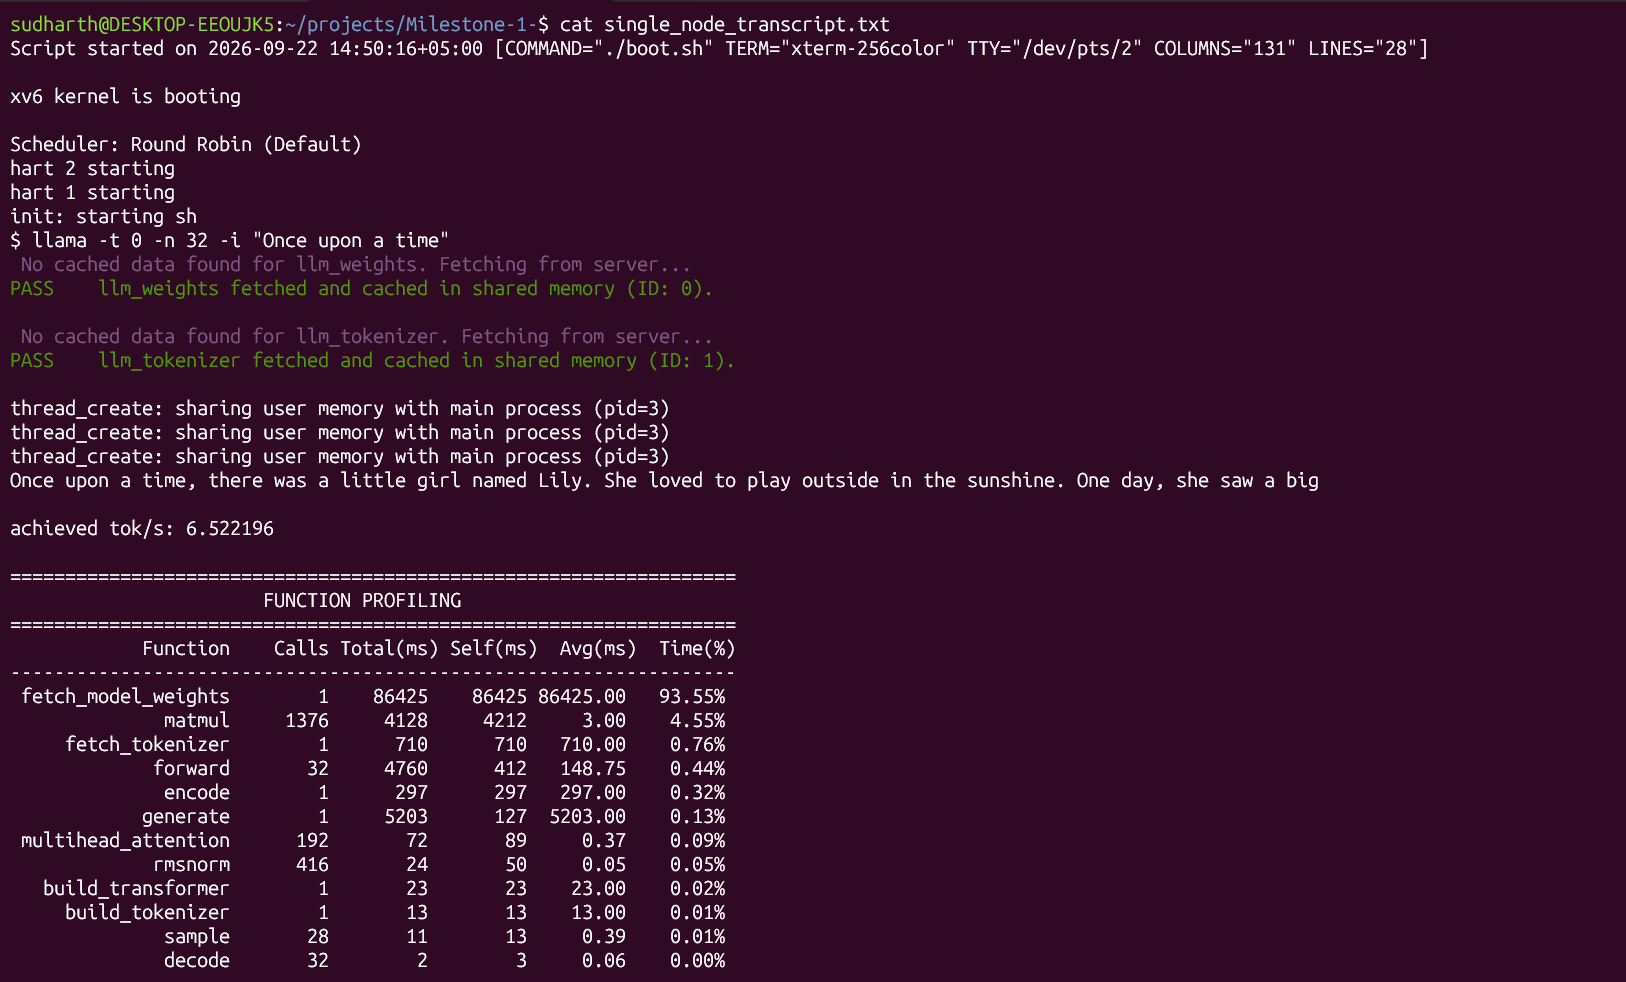
\includegraphics[width=\textwidth]{figures/transcript_single.png}

\caption{Single-node transcript showing generated text.}
\end{figure}

\begin{figure}[H]
\centering
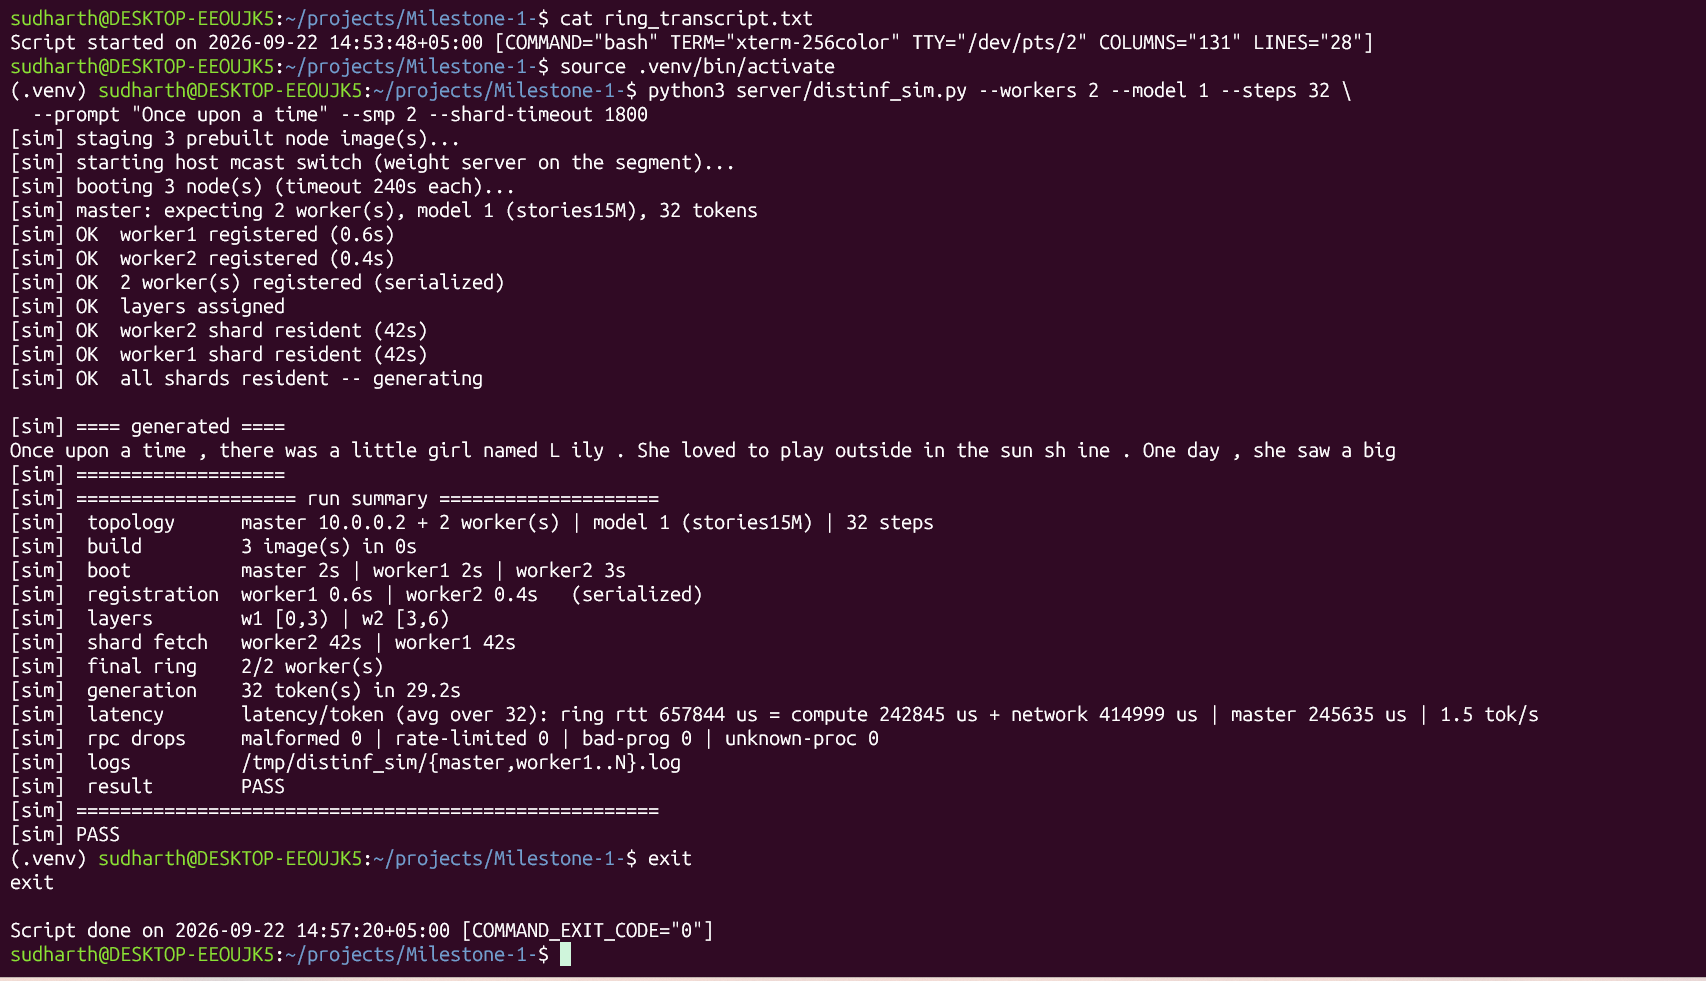
\includegraphics[width=\textwidth]{figures/transcript_ring2.png}

\caption{Multi-node ring (2 workers): workers registering and generated text.}
\end{figure}


\begin{figure}[H]
\centering
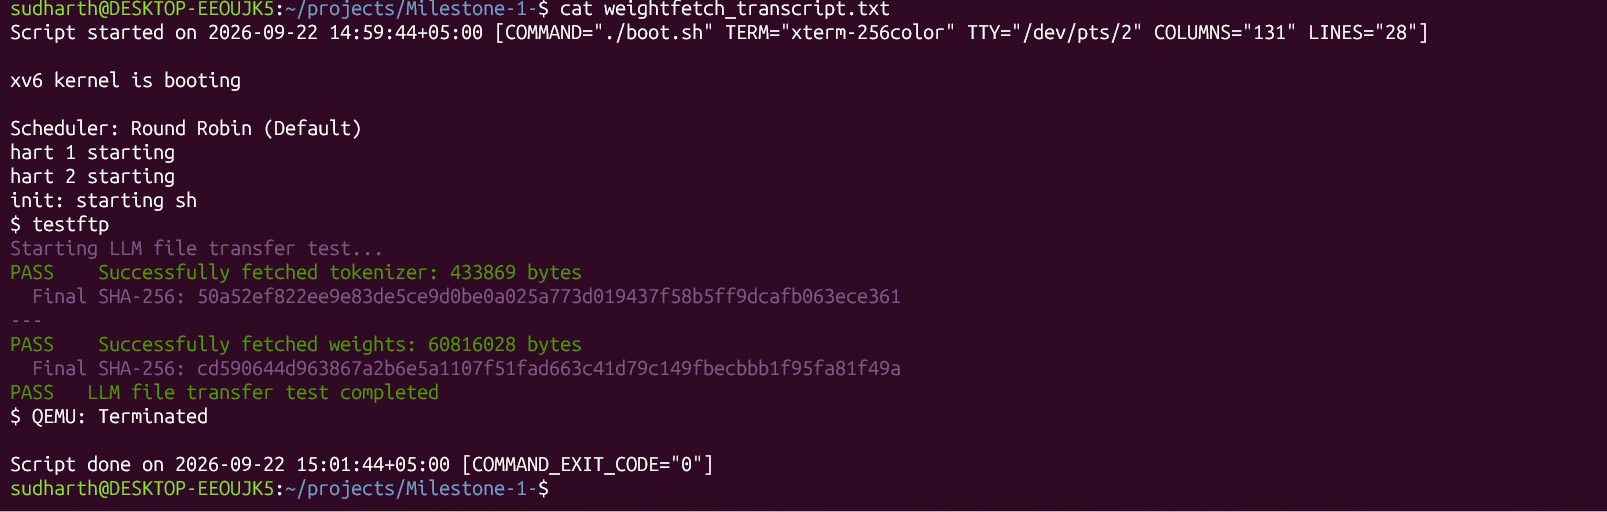
\includegraphics[width=\textwidth]{figures/transcript_weightfetch.png}

\caption{Weight-fetch path: \texttt{testftp} showing bytes transferred.}
\end{figure}


\subsection{Commit Log}

The following commits record the project's progress:
\begin{lstlisting}[language=,basicstyle=\ttfamily\footnotesize]
1f6ae005  Milestone 1: Add F7e/F7f ring charts, 3-worker transcript,
          fix Obs 8, AI Use heading, ring disclaimer
0f7b2fc   Milestone 1: Complete report, figures, runbook,
          transcripts, observations
dd166bf   Initial commit
\end{lstlisting}

\subsection{AI Use}

AI tools (DeepSeek and Claude) were used only for support: DeepSeek for debugging when stuck, and Claude as a reviewer for feedback on the draft. All technical work --- running the three configurations, capturing transcripts, disassembling the kernel, reading the source, writing the report, and building the figures --- was done by the team. All technical claims were verified against the source and binary by the team.

\end{document}